% !TeX root = RJwrapper.tex
\title{PubChemR: An R Package for Accessing Chemical Data from PubChem}


\author{by Selcuk Korkmaz, Bilge Eren Yamasan, and Dincer Goksuluk}

\maketitle

\abstract{%
Chemical data is a cornerstone in the fields of chemistry, pharmacology, bioinformatics, and environmental science. The PubChemR package provides a comprehensive R interface to the PubChem database, which is one of the largest and most complete repositories of chemical data. This package simplifies the process of querying and retrieving chemical information, including compound structures, properties, biological activities, and more, directly from within R. By leveraging PubChemR, users can programmatically access a wealth of chemical data, which is essential for research and analysis in the chemical sciences. The package supports various functionalities such as searching by chemical identifiers, downloading chemical structures, and retrieving bioassay results, among others. PubChemR is designed to be user-friendly, providing a intuitive experience for R users ranging from academic researchers to practitioners across various scientific disciplines. This paper presents the capabilities of PubChemR, demonstrates its use through practical examples, and discusses its potential impact on chemical data analysis.
}

\hypertarget{introduction}{%
\section{Introduction}\label{introduction}}

Chemical data serves as a foundational element in a wide spectrum of scientific research fields, from pharmacology and medicinal chemistry to materials science and environmental studies. The ability to access, query, and manipulate chemical information efficiently is essential for researchers and practitioners who rely on data-driven methodologies to advance their work. PubChem, hosted by the National Center for Biotechnology Information (NCBI), stands as one of the largest publicly available repositories of chemical data, offering free access to an abundance of information on chemical substances, compounds, and biological activities (Wang et al. 2009, 2012; Chen, Wild, and Guha 2009; Li et al. 2010; Kim et al. 2016).

The \CRANpkg{PubChemR} package for R provides a comprehensive interface to the PubChem database, allowing users to programmatically retrieve and utilize chemical data within the R environment (Korkmaz, Yamasan, and Goksuluk 2024). This integration facilitates a more streamlined workflow for scientists who use R for statistical analysis, data visualization, and computational modeling. By utilizing the \CRANpkg{PubChemR} package, users can perform a variety of tasks such as searching for chemical substances, fetching compound properties, and obtaining assay data for bioactivity analysis.

Among the extensive range of R packages used in scientific research, \CRANpkg{webchem} (Szöcs et al. 2020) and \BIOpkg{ChemmineR} (Cao et al. 2008) have been important for accessing chemical databases. \BIOpkg{ChemmineR} provides tools for cheminformatics in R, enabling detailed handling and analysis of chemical data. \CRANpkg{webchem} supports access to multiple chemical databases. Additionally, other notable packages like \CRANpkg{rcdk}, \BIOpkg{ChemmineOB}, \BIOpkg{BridgeDbR}, \BIOpkg{RMassBank}, and \BIOpkg{rgoslin} offer robust functionalities for chemical data manipulation and analysis. The \CRANpkg{rcdk} package interfaces with the Chemistry Development Kit (CDK), providing molecular structure parsing and descriptor calculation (Guha 2007). \BIOpkg{ChemmineOB} interfaces with OpenBabel for chemical format conversions and molecular property calculations (Horan and Girke 2024). \BIOpkg{BridgeDbR} facilitates identifier mapping across biological databases, enhancing data integration (Leemans et al. 2024). \BIOpkg{RMassBank} supports the creation and handling of mass spectrometry databases, crucial for compound identification (Stravs et al. 2013). \BIOpkg{rgoslin} ensures accurate lipid nomenclature in lipidomics studies (Kopczynski et al. 2020).

However, when it comes to direct interaction with the PubChem database, these packages have limitations, often requiring users to work through complex API documentation or use additional tools. To address these issues, \CRANpkg{PubChemR}, designed specifically for the PubChem database, complements the functionalities of these packages. It simplifies accessing chemical data from PubChem, using functions that make API interactions more straightforward. Users can retrieve data easily by calling these functions with the right parameters. Unlike \CRANpkg{webchem}, which works with various databases, and \BIOpkg{ChemmineR}, which covers a wide range of cheminformatics tasks, \CRANpkg{PubChemR} is focused solely on PubChem, allowing for more efficient and targeted data interactions.

Here, we introduce \CRANpkg{PubChemR}, detailing its functionality, design principles, and potential use cases. We will demonstrate how \CRANpkg{PubChemR} can be utilized to enhance research workflows and provide examples of its application in real-world scenarios. By the end of this paper, readers will be equipped with the knowledge to integrate \CRANpkg{PubChemR} into their data analysis toolkit, unlocking the potential to drive forward chemical and biological research with the power of R.

\hypertarget{design}{%
\section{Design}\label{design}}

The design of \CRANpkg{PubChemR} is driven by the need for a seamless and intuitive interface for R users to access the vast chemical data available in the PubChem database. Our design principles focus on simplicity, efficiency, and robustness:

\begin{itemize}
\item
  \textbf{Simplicity:} The package is designed to minimize the complexity of interacting with the PubChem API. Functions are named and structured to be self-explanatory, allowing users to intuitively understand their purposes.
\item
  \textbf{Efficiency:} Considering the extensive size of the PubChem database, we optimized \CRANpkg{PubChemR} for speed and minimal resource consumption. Our design includes efficient handling of API calls and data processing.
\item
  \textbf{Robustness:} The package is designed to handle a wide range of user queries, from simple compound searches to complex data extractions. Exception handling and error reporting are integral, ensuring users are informed of issues in their queries or data processing.
\end{itemize}

\hypertarget{implementation}{%
\section{Implementation}\label{implementation}}

The implementation of \CRANpkg{PubChemR} involved several key steps:

\begin{itemize}
\item
  \textbf{API Integration:} We integrated the PubChem API using R's HTTP client capabilities. This involved mapping the PubChem's RESTful services into R functions.
\item
  \textbf{Data Processing:} The raw data from PubChem API calls are processed and transformed into user-friendly R data structures such as data frames and lists.
\item
  \textbf{Function Development:} Each function in \CRANpkg{PubChemR} corresponds to a specific type of query or data retrieval from the PubChem database, with parameters allowing for flexible and targeted searches.
\item
  \textbf{Testing and Validation:} We performed rigorous testing to ensure accuracy and efficiency using the testthat package for unit testing each function. This approach helps us define and verify expected behavior, catch errors, and integrate well with our workflow, thereby maintaining high code quality and reliability.
\end{itemize}

\hypertarget{use-cases}{%
\section{Use cases}\label{use-cases}}

The \CRANpkg{PubChemR} package interfaces with the PubChem database through URL syntax, with each query within this syntax serving as an argument in the designated function (Figure 1).

\begin{figure}
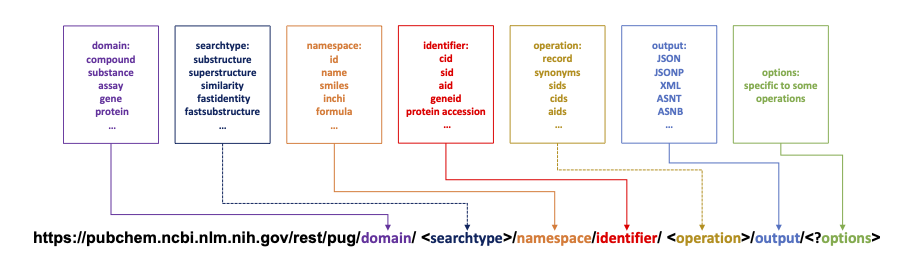
\includegraphics[width=1\linewidth,height=0.2\textheight]{figures/Figure_1} \caption{Interfacing the PubChem's PUG-REST database with the PubChemR package through URL syntax: utilizing queries as function arguments}\label{fig:figure1}
\end{figure}

The functions in \CRANpkg{PubChemR} are designed with flexibility in mind, allowing users to specify the type of information they need and the format in which they wish to receive it. For instance, data can be returned as R objects like data frames or lists, ready for analysis.

\CRANpkg{PubChemR} pacakage can be installed from CRAN (The Comprehensive R Archive Network) and loaded as follow:

\begin{verbatim}
# install.packages("PubChemR", repos = "http://cran.us.r-project.org")
library("PubChemR")
\end{verbatim}

The package is currently in a state of active development. The latest version in development can be accessed via GitHub (\url{https://github.com/selcukorkmaz/PubChemR}). This paper was composed utilizing \CRANpkg{PubChemR} version 2.1.

Most functions in the package require three main arguments; domain, namespace, and identifier.

\textbf{1. Domain:} This represents the primary classification within the PubChem system that dictates the type of data being accessed. Examples of domains include ``substance,'' ``compound,'' ``assay,'' ``gene,'' and others. Each domain encapsulates specific types of scientific data, such as chemical compounds or genetic information.

\textbf{2. Namespace:} Within each domain, the namespace further specifies the method or criteria for querying the data. It acts as a sub-category within the domain that allows for more refined searches. For instance, in the compound domain, namespaces can be specific identifiers like ``cid'' for compound ID, or ``name'' for the compound's common name, among others.

\textbf{3. Identifier:} These are the actual data values used to perform the query. Identifiers can be vector of positive integers (e.g.~cid, sid, aid) or strings (e.g.~name, smiles, source, inchikey, formula). They are the key pieces of information that pinpoint the exact record or set of records to be retrieved from the database.

Additionally, the optional arguments ``operation'' and ``searchtype'' play crucial roles in refining the scope and focus of data queries. The ``operation'' argument specifies the type of data processing or retrieval task that should be performed on the identified records. For instance, operations can range from fetching complete data records to retrieving specific properties or summaries of compounds, genes, or assays. This flexibility allows users to access both broad overviews and detailed attributes of database entries according to their research needs. Meanwhile, the ``searchtype'' argument defines the method of search being employed. It could be a structured search, such as substructure or similarity search, which is essential for identifying compounds with particular chemical structures or features. These optional arguments enhance the API's versatility, enabling researchers to tailor queries more precisely and retrieve data that best fits their experimental and analytical requirements. For more detailed information, please refer to the official documentation at \url{https://pubchem.ncbi.nlm.nih.gov/docs/pug-rest}.

Table 1 provides detailed information about four key arguments: ``domain,'' ``searchtype,'' ``namespace,'' and ``operation.'' This table is designed to help users understand how to effectively utilize these components to customize queries within the PubChemR package.

\begin{longtable}[]{@{}
  >{\raggedright\arraybackslash}p{(\columnwidth - 6\tabcolsep) * \real{0.2500}}
  >{\raggedright\arraybackslash}p{(\columnwidth - 6\tabcolsep) * \real{0.2500}}
  >{\raggedright\arraybackslash}p{(\columnwidth - 6\tabcolsep) * \real{0.2500}}
  >{\raggedright\arraybackslash}p{(\columnwidth - 6\tabcolsep) * \real{0.2500}}@{}}
\toprule\noalign{}
\begin{minipage}[b]{\linewidth}\raggedright
domain
\end{minipage} & \begin{minipage}[b]{\linewidth}\raggedright
searchtype
\end{minipage} & \begin{minipage}[b]{\linewidth}\raggedright
namespace
\end{minipage} & \begin{minipage}[b]{\linewidth}\raggedright
operation
\end{minipage} \\
\midrule\noalign{}
\endhead
\bottomrule\noalign{}
\endlastfoot
substance & - & sid, sourceid/\textless source id\textgreater, sourceall/\textless source name\textgreater, name, \textless xref\textgreater, listkey & record, synonyms, sids, cids, aids, assaysummary, classification, \textless xrefs\textgreater, description \\
compound & \textless structure search\textgreater{} = \{substructure, superstructure, similarity, identity\}/\{smiles, inchi, sdf, cid\} \textless fast search\textgreater{} = \{fastidentity, fastsimilarity\_2d, fastsimilarity\_3d, fastsubstructure, fastsuperstructure\}/\{smiles, smarts, inchi, sdf, cid\}, fastformula & cid, name, smiles, inchi, sdf, inchikey, formula, \textless structure search\textgreater, \textless xref\textgreater, listkey, \textless fast search\textgreater{} & record, \textless compound property\textgreater, synonyms, sids, cids, aids, assaysummary, classification, \textless xrefs\textgreater, description, conformers \\
assay & - & aid, listkey, type/\textless assay type\textgreater, sourceall/\textless source name\textgreater, target/\textless assay target\textgreater, activity/\textless activity column name\textgreater{} & record, concise, aids, sids, cids, description, targets/\textless target type\textgreater, \textless doseresponse\textgreater, summary, classification \\
gene & - & geneid, genesymbol, synonym & summary, aids, concise, pwaccs \\
protein & - & accession, gi, synonym & summary, aids, concise, pwaccs \\
pathway & - & pwacc & summary, cids, geneids, accessions \\
taxonomy & - & taxid, synonym & summary, aids \\
cell & - & cellacc, synonym & summary, aids \\
\end{longtable}

Table 1: Overview of key arguments in the PubChemR package

In the following sections, we will explore each function in detail, examining the parameters they accept, the type of data they return, and providing examples to illustrate their use. These examples will serve as a guide for users to understand how to effectively utilize the \CRANpkg{PubChemR} package to access and manipulate chemical and biological data for their specific needs.

First, we will concentrate on three primary functions, each focusing on a specific domain: \texttt{get\_compounds} to retrieve compound data, \texttt{get\_substances} to extract substance data, and \texttt{get\_assays} to fetch assay data. These functions are capable of handling multiple queries simultaneously and return a \emph{PubChemInstanceList} class. This is a specialized class specifically created for these functions to manage the complex PubChem data efficiently. After utilizing each of these functions, we will employ the \texttt{instance} function. This function is designed to retrieve detailed information about a compound from a \emph{PubChemInstanceList}. It provides comprehensive details about the specific compound, including its instance details (i.e., slots). Finally, we will implement the \texttt{retrieve} function with the relevant slots to extract specific data elements from the compound data. This approach ensures that we can precisely access the required information from the vast amount of data available, thereby enhancing the efficiency and effectiveness of our data analysis process.

Next, we will fetch a variety of compound properties, such as molecular weight, chemical formula, isomeric SMILES, and more, using the \texttt{get\_properties} function. Additionally, we will focus on two functions for downloading data from the PubChem database: \texttt{get\_sdf} and \texttt{download.} The \texttt{get\_sdf} function is specifically designed to download chemical structure data in the widely recognized Structure Data File (SDF) format. The \texttt{download} function streamlines the process of accessing and downloading content from the PubChem database.

Finally, we will introduce two new functions: \texttt{get\_pug\_rest} and \texttt{get\_pug\_view.} The \texttt{get\_pug\_rest} function provides a direct and efficient method for accessing a wide range of chemical data. In contrast, the \texttt{get\_pug\_view} function is designed to offer access to detailed summary reports and additional information that is not usually included in the primary PubChem Substance, Compound, or BioAssay records.

\hypertarget{retrieve-compund-information}{%
\subsection{Retrieve Compund Information}\label{retrieve-compund-information}}

The \texttt{get\_compounds} function allows R users to retrieve compound information from the PubChem database. This function specifically targets retrieving compound-related information. This specialized focus is crucial for users who require direct and efficient access to detailed compound data, a common need in various fields of chemical research and analysis. Below, we will demonstrate how to retrieve compound data using different namespaces:

\textbf{a. Retrieving Compound Information by Name:} The \texttt{get\_compounds} function simplifies the process of retrieving detailed compound information by using common compound names. This feature is particularly beneficial in scenarios where the specific CIDs of compounds are unknown or in educational contexts where common names are more frequently used. It simplifies the process of data retrieval for users who may not be familiar with the technical identifiers of compounds but are well-versed with their common or commercial names.

Consider the following example where the \texttt{get\_compounds} function is employed to fetch data for compounds using their common names:

\begin{verbatim}
compounds <- get_compounds(identifier = c("aspirin", "caffeine", "glucose"), namespace = "name") 
compounds
\end{verbatim}

\begin{verbatim}
#> 
#>  An object of class 'PubChemInstanceList'
#> 
#>  Number of instances: 3
#>   - Domain: Compound
#>   - Namespace: Name
#>   - Identifier(s): aspirin, caffeine, ... and 1 more.
#> 
#>  * Run 'instance(...)' function to extract specific instances from the complete list, and
#>    'request_args(...)' to see all the requested instance identifiers.
#>  * See ?instance and ?request_args for details.
\end{verbatim}

The \texttt{request\_args} function can be executed to view all the requested instance identifiers:

\begin{verbatim}
request_args(object = compounds)
\end{verbatim}

\begin{verbatim}
#> $namespace
#> [1] "name"
#> 
#> $identifier
#> [1] "aspirin"  "caffeine" "glucose" 
#> 
#> $domain
#> [1] "compound"
#> 
#> $operation
#> NULL
#> 
#> $options
#> NULL
#> 
#> $searchtype
#> NULL
\end{verbatim}

To retrieve detailed information about a specific compound (e.g.~aspirin), we can use the \texttt{instance} function on the result:

\begin{verbatim}
compound_aspirin <- instance(object = compounds, .which = "aspirin")
compound_aspirin
\end{verbatim}

\begin{verbatim}
#> 
#>  An object of class 'PubChemInstance'
#> 
#>  Request Details:  
#>   - Domain: Compound
#>   - Namespace: Name
#>   - Identifier: aspirin
#> 
#>  Instance Details:  
#>   - id (1): [<named list>] id
#>   - atoms (2): [<named list>] aid, element
#>   - bonds (3): [<named list>] aid1, aid2, order
#>   - coords (1): [<unnamed list>] 
#>   - charge (1): [<unnamed numeric>] 
#>   - props (22): [<unnamed list>] 
#>   - count (10): [<named numeric>] heavy_atom, atom_chiral, atom_chiral_def, atom_chiral_undef, ...
#> 
#>  NOTE: Run getter function 'retrieve()' with element name above to extract data from corresponding list. 
#>        See ?retrieve for details.
\end{verbatim}

The \texttt{instance} function retrieves detailed information about the specific compound, including its various components (known as slots). In this example, the compound has seven slots: \texttt{id}, \texttt{atoms}, \texttt{bonds}, \texttt{coords}, \texttt{charge}, \texttt{props}, and \texttt{count}. To extract specific data elements from the compound data, we can use the \texttt{retrieve} function with the relevant slots. For example, using the \emph{props} slot extracts detailed properties of the compound, including information such as label, name, data type, release, value, implementation, version, software, and source. This comprehensive information covers various physical, chemical, and structural properties of the compound.

\begin{verbatim}
retrieve(object = compound_aspirin, .slot = "props", .to.data.frame = TRUE)
\end{verbatim}

\begin{verbatim}
#> # A tibble: 22 x 11
#>    Identifier label name  datatype release value implementation version software
#>    <chr>      <chr> <chr> <chr>    <chr>   <chr> <chr>          <chr>   <chr>   
#>  1 aspirin    Comp~ Cano~ 5        2021.1~ 1     <NA>           <NA>    <NA>    
#>  2 aspirin    Comp~ <NA>  7        2021.1~ 212   E_COMPLEXITY   3.4.8.~ Cactvs  
#>  3 aspirin    Count Hydr~ 5        2021.1~ 4     E_NHACCEPTORS  3.4.8.~ Cactvs  
#>  4 aspirin    Count Hydr~ 5        2021.1~ 1     E_NHDONORS     3.4.8.~ Cactvs  
#>  5 aspirin    Count Rota~ 5        2021.1~ 3     E_NROTBONDS    3.4.8.~ Cactvs  
#>  6 aspirin    Fing~ SubS~ 16       2021.1~ 0000~ E_SCREEN       3.4.8.~ Cactvs  
#>  7 aspirin    IUPA~ Allo~ 1        2021.1~ 2-ac~ <NA>           2.7.0   Lexiche~
#>  8 aspirin    IUPA~ CAS-~ 1        2021.1~ 2-ac~ <NA>           2.7.0   Lexiche~
#>  9 aspirin    IUPA~ Mark~ 1        2021.1~ 2-ac~ <NA>           2.7.0   Lexiche~
#> 10 aspirin    IUPA~ Pref~ 1        2021.1~ 2-ac~ <NA>           2.7.0   Lexiche~
#> # i 12 more rows
#> # i 2 more variables: source <chr>, parameters <chr>
\end{verbatim}

\textbf{b. Retrieving Compound Information by CID:} The \texttt{get\_compounds} function can be used to extract detailed compound data utilizing CIDs. This feature is particularly advantageous for researchers who require precise and comprehensive data on specific compounds. By inputting a vector of CIDs, users can quickly access a vast amount of information for their research needs.

Here's an illustrative example demonstrating the use of \texttt{get\_compounds} to obtain data for a set of compounds using their CIDs:

\begin{verbatim}
compounds <- get_compounds(identifier = c(2244, 305), namespace = "cid") 
compounds
\end{verbatim}

\begin{verbatim}
#> 
#>  An object of class 'PubChemInstanceList'
#> 
#>  Number of instances: 2
#>   - Domain: Compound
#>   - Namespace: CID
#>   - Identifier(s): 2244, 305
#> 
#>  * Run 'instance(...)' function to extract specific instances from the complete list, and
#>    'request_args(...)' to see all the requested instance identifiers.
#>  * See ?instance and ?request_args for details.
\end{verbatim}

Similarly, we can use the \texttt{instance} function on the result to retrieve detailed information about CID 2244:

\begin{verbatim}
compound_2244 <- instance(object = compounds, .which = 2244)
compound_2244
\end{verbatim}

\begin{verbatim}
#> 
#>  An object of class 'PubChemInstance'
#> 
#>  Request Details:  
#>   - Domain: Compound
#>   - Namespace: CID
#>   - Identifier: 2244
#> 
#>  Instance Details:  
#>   - id (1): [<named list>] id
#>   - atoms (2): [<named list>] aid, element
#>   - bonds (3): [<named list>] aid1, aid2, order
#>   - coords (1): [<unnamed list>] 
#>   - charge (1): [<unnamed numeric>] 
#>   - props (22): [<unnamed list>] 
#>   - count (10): [<named numeric>] heavy_atom, atom_chiral, atom_chiral_def, atom_chiral_undef, ...
#> 
#>  NOTE: Run getter function 'retrieve()' with element name above to extract data from corresponding list. 
#>        See ?retrieve for details.
\end{verbatim}

Similar to the previous section, we can use the \texttt{retrieve} function with the element names (i.e.~slots) mentioned above to extract specific data sections.

\textbf{c.~Advanced Search with SMILES:} In cheminformatics, the Simplified Molecular Input Line Entry System (SMILES) is a widely-used method for representing chemical structures. The \texttt{get\_compounds} function package adeptly handles queries based on SMILES strings, enabling users to search for compounds by their structural characteristics. The main advantage of using SMILES is their precise representation of molecular structures, unlike CIDs or chemical names that can be ambiguous or inapplicable.

Consider the following example where the \texttt{get\_compounds} function is used to search for compounds using their SMILES strings:

\begin{verbatim}
compounds_by_smiles <- get_compounds(identifier = c("CC(=O)OC1=CC=CC=C1C(=O)O", 
                                                    "CN1C=NC2=C1C(=O)N(C(=O)N2C)C"), 
                                     namespace = "smiles")  
compounds_by_smiles
\end{verbatim}

\begin{verbatim}
#> 
#>  An object of class 'PubChemInstanceList'
#> 
#>  Number of instances: 2
#>   - Domain: Compound
#>   - Namespace: SMILES
#>   - Identifier(s): CC(=O)OC1=CC=CC=C1C(=O)O, CN1C=NC2=C1C(=O)N(C(=O)N2C)C
#> 
#>  * Run 'instance(...)' function to extract specific instances from the complete list, and
#>    'request_args(...)' to see all the requested instance identifiers.
#>  * See ?instance and ?request_args for details.
\end{verbatim}

In this example, compounds\_by\_smiles object is a \emph{PubChemInstanceList} containing data for compounds that correspond to the provided SMILES strings. The strings ``CC(=O)OC1=CC=CC=C1C(=O)O'' and ``CN1C=NC2=C1C(=O)N(C(=O)N2C)C'' represent the molecular structures of aspirin and caffeine, respectively. The function returns a \emph{PubChemInstanceList} where each element contains comprehensive information about these compounds.

Let's only access data for \emph{CC(=O)OC1=CC=CC=C1C(=O)O} using the instance function.

\begin{verbatim}
compound_smiles <- instance(object = compounds_by_smiles, .which = "CC(=O)OC1=CC=CC=C1C(=O)O")
compound_smiles
\end{verbatim}

\begin{verbatim}
#> 
#>  An object of class 'PubChemInstance'
#> 
#>  Request Details:  
#>   - Domain: Compound
#>   - Namespace: SMILES
#>   - Identifier: CC(=O)OC1=CC=CC=C1C(=O)O
#> 
#>  Instance Details:  
#>   - id (1): [<named list>] id
#>   - atoms (2): [<named list>] aid, element
#>   - bonds (3): [<named list>] aid1, aid2, order
#>   - coords (1): [<unnamed list>] 
#>   - charge (1): [<unnamed numeric>] 
#>   - props (22): [<unnamed list>] 
#>   - count (10): [<named numeric>] heavy_atom, atom_chiral, atom_chiral_def, atom_chiral_undef, ...
#> 
#>  NOTE: Run getter function 'retrieve()' with element name above to extract data from corresponding list. 
#>        See ?retrieve for details.
\end{verbatim}

Finally, we can utilize the \texttt{retrieve} function to access data in each slot of the \emph{compound\_smiles} object, as demonstrated earlier.

\hypertarget{retrieve-substance-information}{%
\subsection{Retrieve Substance Information}\label{retrieve-substance-information}}

The \texttt{get\_substances} function is for researchers looking to explore the extensive substance records in the PubChem database. PubChem's definition of substances encompasses a broad spectrum of chemical entities, ranging from unique samples of individual chemical compounds to complex mixtures. These substances often manifest in diverse forms, including but not limited to different salts, isotopes, complexes, or combinations of various compounds.

The \texttt{get\_substances} function is designed to meet the specific requirements of accessing a wide range of substance records. It uses unique substance identifiers (SIDs) for each substance in PubChem, allowing users to easily and accurately retrieve detailed information. This feature is especially important in situations where understanding the differences between various forms or versions of a compound is critical, such as in drug research, managing chemical databases, or meeting regulatory standards.

In the following example, we will retrieve substance data for three substances using their SIDs:

\begin{itemize}
\item
  Aspirin (SID: 103164874): Aspirin, also known as acetylsalicylic acid, is widely used as an analgesic to relieve pain, reduce fever, and act as an anti-inflammatory medication. As a substance, it encompasses various forms and preparations of aspirin available from different sources.
\item
  Caffeine (SID: 403385742): Caffeine is a central nervous system stimulant commonly found in coffee, tea, and various energy drinks. As a substance, it includes different sources and formulations of caffeine beyond its pure chemical structure.
\item
  Glucose (SID: 403435554): Glucose is a simple sugar that serves as a primary energy source for living organisms. As a substance, it includes various forms and sources of glucose, providing detailed information beyond the pure compound.
\end{itemize}

Using the \texttt{get\_substances} function, we can access detailed records for these substances in the PubChem database by providing their SIDs.

\begin{verbatim}
substances <- get_substances(identifier = c(103164874, 403385742, 403435554), 
                             namespace = "sid") 
substances
\end{verbatim}

\begin{verbatim}
#> 
#>  An object of class 'PubChemInstanceList'
#> 
#>  Number of instances: 3
#>   - Domain: Substance
#>   - Namespace: SID
#>   - Identifier(s): 103164874, 403385742, ... and 1 more.
#> 
#>  * Run 'instance(...)' function to extract specific instances from the complete list, and
#>    'request_args(...)' to see all the requested instance identifiers.
#>  * See ?instance and ?request_args for details.
\end{verbatim}

Next, let's fetch detailed substance information for glucose (SID: 403435554). First, we need to run the instance function to see the slots that contain substance data:

\begin{verbatim}
instance(object = substances, .which = 403435554)
\end{verbatim}

\begin{verbatim}
#> 
#>  Substance Data from PubChem Database 
#> 
#>  Request Details:  
#>   - Domain: Substance
#>   - Namespace: SID
#>   - Identifier: 403435554
#> 
#>  Number of substances retrieved: 1
#> 
#>  Substances contain data within following slots; 
#>   - sid (2): [<named numeric>] id, version
#>   - source (1): [<named list>] db
#>   - xref (3): [<unnamed list>] 
#>   - compound (2): [<unnamed list>] 
#> 
#>  NOTE: Run getter function 'retrieve()' with element name above to extract data from corresponding list. 
#>        See ?retrieve for details.
\end{verbatim}

The output shows four slots that contain substance data for glucose. We can retrieve data from each slot using the \texttt{retrieve} function. For example, we can extract detailed compound information, such as the compound ID, atom IDs and elements, charges, bond details, and coordinates for molecular structure visualization:

\begin{verbatim}
retrieve(object = substances, .which = 403435554, .slot = "compound", .to.data.frame = FALSE)
\end{verbatim}

\begin{verbatim}
#> $Identifier
#> [1] 403435554
#> 
#> [[2]]
#> [[2]]$id
#> type 
#>    0 
#> 
#> [[2]]$atoms
#> [[2]]$atoms$aid
#>  [1]  1  2  3  4  5  6  7  8  9 10 11 12 13 14 15 16
#> 
#> [[2]]$atoms$element
#>  [1] 8 8 8 8 8 6 6 8 6 6 6 6 1 1 1 1
#> 
#> 
#> [[2]]$bonds
#> [[2]]$bonds$aid1
#>  [1]  6  7  7  8  9  9 10 10 10 11 11 11 12 12 12 12
#> 
#> [[2]]$bonds$aid2
#>  [1]  5  6 13  7  4  8  3  9 16  2 10 15  1  7 11 14
#> 
#> [[2]]$bonds$order
#>  [1] 1 1 1 1 1 1 1 1 1 1 1 1 1 1 1 1
#> 
#> 
#> [[2]]$coords
#> [[2]]$coords[[1]]
#> [[2]]$coords[[1]]$type
#> [1] 1 3
#> 
#> [[2]]$coords[[1]]$aid
#>  [1]  1  2  3  4  5  6  7  8  9 10 11 12 13 14 15 16
#> 
#> [[2]]$coords[[1]]$conformers
#> [[2]]$coords[[1]]$conformers[[1]]
#> [[2]]$coords[[1]]$conformers[[1]]$x
#>  [1] -1.1936  0.3873  2.0000  2.0000 -2.0000 -1.1936 -0.3873  0.3873  1.1936
#> [10]  1.1936  0.3873 -0.3873 -0.9849 -0.9129 -0.1439  1.7192
#> 
#> [[2]]$coords[[1]]$conformers[[1]]$y
#>  [1] -0.4492 -1.3794 -0.4492  1.3794  0.9143  1.3794  0.9143  1.3794  0.9143
#> [10]  0.0144 -0.4492  0.0144  0.8106  0.3182 -0.7429  0.3168
#> 
#> [[2]]$coords[[1]]$conformers[[1]]$style
#> [[2]]$coords[[1]]$conformers[[1]]$style$annotation
#> [1] 6 5 6 5
#> 
#> [[2]]$coords[[1]]$conformers[[1]]$style$aid1
#> [1]  7 10 11 12
#> 
#> [[2]]$coords[[1]]$conformers[[1]]$style$aid2
#> [1] 13 16 15 14
#> 
#> 
#> 
#> 
#> 
#> 
#> [[2]]$charge
#> [1] 0
#> 
#> 
#> [[3]]
#> [[3]]$id
#> [[3]]$id$type
#> [1] 1
#> 
#> [[3]]$id$id
#>  cid 
#> 5793
\end{verbatim}

Besides SIDs, the function supports additional namespaces such as sourceid, sourceall, name, xref, and listkey. This flexibility enables researchers to access substance records from a range of perspectives, depending on their available data or specific requirements.

\hypertarget{retrieve-assay-information}{%
\subsection{Retrieve Assay Information}\label{retrieve-assay-information}}

The \texttt{get\_assays} function is another key function for researchers needing detailed biological assay information from the PubChem database. These assays, essential for drug discovery, toxicology, and pharmacology, measure biological activities of substances. The function simplifies accessing this data, crucial for bioinformatics and cheminformatics (Korkmaz 2020; Yamasan and Korkmaz 2024). It enables customized queries in the PubChem database, allowing users to explore a wide range of assay data, including drug efficacy and toxicity. Its versatility in handling different parameters facilitates a specific data retrieval approach.

The utility of the \texttt{get\_assays} function extends across multiple research scenarios. In drug discovery, It enables researchers to explore assays related to potential drug compounds, aiding in the comprehension of their efficacy and safety profiles. In toxicological studies, the function is key in acquiring insights into the toxic effects of diverse substances.

In the field of scientific research, particularly in areas such as pharmacology, toxicology, and biochemistry, researchers frequently encounter specific assays that are of interest to their studies. These assays are often identified by their Assay IDs (AIDs), which are referenced in scientific literature or various databases. The get\_assays function provides a direct and efficient means for researchers to access comprehensive information about these particular assays.

Utilizing the \texttt{get\_assays} function, researchers can input a vector of AIDs to retrieve detailed data about each corresponding assay. This functionality is especially beneficial for those who need to analyze and interpret assay data as part of their research projects or for educational purposes.

Consider the following practical example where we retrieve assay data from PubChem using their AIDs.

First, we use the \texttt{get\_assays} function to retrieve data for the specified assays. The identifier parameter is a vector of AIDs (485314, 485341, 504466, 624202, and 651820), and the namespace parameter specifies that the identifiers are AIDs.

\begin{verbatim}
assays <- get_assays(identifier = c(485314, 485341, 504466, 624202, 651820), 
                     namespace = "aid") 
assays
\end{verbatim}

\begin{verbatim}
#> 
#>  An object of class 'PubChemInstanceList'
#> 
#>  Number of instances: 5
#>   - Domain: Assay
#>   - Namespace: AID
#>   - Identifier(s): 485314, 485341, ... and 3 more.
#> 
#>  * Run 'instance(...)' function to extract specific instances from the complete list, and
#>    'request_args(...)' to see all the requested instance identifiers.
#>  * See ?instance and ?request_args for details.
\end{verbatim}

The output shows that the assays object is of class `\emph{PubChemInstanceList}' and contains data for 5 assays identified by their AIDs. It includes information about the number of instances (5 in this case), the domain (Assay), the namespace (AID), and the specific identifiers. The output also provides hints on how to proceed further.

Now, we can use the \texttt{instance} function to extract specific instances from the complete list. For example, the following code extracts the detailed data for the assay with identifier 485314 from the list of assays:

\begin{verbatim}
assay_485314 <- instance(object = assays, .which = 485314)
assay_485314
\end{verbatim}

\begin{verbatim}
#> 
#>  An object of class 'PubChemInstance'
#> 
#>  Request Details:  
#>   - Domain: Assay
#>   - Namespace: AID
#>   - Identifier: 485314
#> 
#>  Instance Details:  
#>   - aid (2): [<named numeric>] id, version
#>   - aid_source (1): [<named list>] db
#>   - name (1): [<unnamed character>] 
#>   - description (3): [<unnamed character>] 
#>   - protocol (1): [<unnamed character>] 
#>   - comment (4): [<unnamed character>] 
#>   - xref (4): [<unnamed list>] 
#>   - results (23): [<unnamed list>] 
#>   - revision (1): [<unnamed numeric>] 
#>   - target (1): [<unnamed list>] 
#>   - activity_outcome_method (1): [<unnamed numeric>] 
#>   - dr (1): [<unnamed list>] 
#>   - grant_number (1): [<unnamed character>] 
#>   - project_category (1): [<unnamed numeric>] 
#> 
#>  NOTE: Run getter function 'retrieve()' with element name above to extract data from corresponding list. 
#>        See ?retrieve for details.
\end{verbatim}

The output provides a detailed view of the assay\_485314 object, which is of class `PubChemInstance'. It includes both request details and instance details

The output also notes that we can use the \texttt{retrieve} function with the element names above to extract data from the corresponding list. For example, we can retrieve the results of the assay, providing detailed data on the outcomes observed during the assay:

\begin{verbatim}
retrieve(object = assays, .which = 485314, .slot = "results")
\end{verbatim}

\begin{verbatim}
#> # A tibble: 41 x 8
#>    Identifier tid   name                 description     type  unit  ac    tc   
#>         <dbl> <chr> <chr>                <chr>           <chr> <chr> <chr> <chr>
#>  1     485314 1     Phenotype            Indicates type~ 4     254   <NA>  <NA> 
#>  2     485314 2     Potency              Concentration ~ 1     5     TRUE  <NA> 
#>  3     485314 3     Efficacy             Maximal effica~ 1     15    <NA>  <NA> 
#>  4     485314 4     Analysis Comment     Annotation/not~ 4     254   <NA>  <NA> 
#>  5     485314 5     Curve_Description    A description ~ 4     254   <NA>  <NA> 
#>  6     485314 6     Fit_LogAC50          The logarithm ~ 1     254   <NA>  <NA> 
#>  7     485314 7     Fit_HillSlope        The Hill slope~ 1     254   <NA>  <NA> 
#>  8     485314 8     Fit_R2               R^2 fit value ~ 1     254   <NA>  <NA> 
#>  9     485314 9     Fit_InfiniteActivity The asymptotic~ 1     15    <NA>  <NA> 
#> 10     485314 10    Fit_ZeroActivity     Efficacy at ze~ 1     15    <NA>  <NA> 
#> # i 31 more rows
\end{verbatim}

By following these steps and using the \texttt{retrieve} function, we can access detailed and specific data from the assay records in PubChem. This comprehensive approach allows researchers to gather all necessary information about assays, aiding in their analysis and research activities.

\hypertarget{retrieve-property-information}{%
\subsection{Retrieve Property Information}\label{retrieve-property-information}}

The \texttt{get\_properties} is another important function for researchers who require access to specific chemical property data from the PubChem database. This function is designed with the aim of simplifying the process of querying PubChem for a variety of compound properties, such as molecular weight, chemical formula, isomeric SMILES, and more. It is particularly useful for those in need of detailed chemical information across a range of compounds.

The \texttt{get\_properties} function allows users to specify a set of properties and the identifiers of the compounds for which these properties are required. The function then queries the PubChem database and retrieves the requested data.

Consider the following practical application of the \texttt{get\_properties} function:

First, we use the \texttt{get\_properties} function to retrieve specific properties for several compounds identified by their names:

\begin{verbatim}
props <- get_properties(
  properties = c("MolecularWeight", "MolecularFormula", "InChI"),
  identifier = c("aspirin", "caffeine", "glucose"),
  namespace = "name"
)
\end{verbatim}

In this example, the \emph{properties} parameter specifies that we want to retrieve the molecular weight, molecular formula, and InChI for each compound. The \emph{identifier} parameter lists the common names of the compounds (aspirin, caffeine, and glucose), and the \emph{namespace} parameter indicates that these identifiers are compound names. The function fetches the specified properties from the PubChem database.

To extract the properties for a specific compound, such as aspirin, we can use the \texttt{retrieve} function:

\begin{verbatim}
retrieve(instance(props, "aspirin"), .slot = NULL)
\end{verbatim}

\begin{verbatim}
#> # A tibble: 1 x 6
#>   Identifier   CID MolecularFormula MolecularWeight InChI               InChIKey
#>   <chr>      <dbl> <chr>            <chr>           <chr>               <chr>   
#> 1 aspirin     2244 C9H8O4           180.16          InChI=1S/C9H8O4/c1~ BSYNRYM~
\end{verbatim}

This tibble shows the identifier (aspirin), CID (2244), molecular formula (C9H8O4), molecular weight (180.16), InChI, and InChIKey.

To combine the properties of all compounds into a single data frame, we set \texttt{.combine.all} as \texttt{TRUE}:

\begin{verbatim}
retrieve(props, .combine.all = TRUE)
\end{verbatim}

\begin{verbatim}
#> # A tibble: 3 x 6
#>   Identifier   CID MolecularFormula MolecularWeight InChI               InChIKey
#>   <chr>      <dbl> <chr>            <chr>           <chr>               <chr>   
#> 1 aspirin     2244 C9H8O4           180.16          InChI=1S/C9H8O4/c1~ BSYNRYM~
#> 2 caffeine    2519 C8H10N4O2        194.19          InChI=1S/C8H10N4O2~ RYYVLZV~
#> 3 glucose     5793 C6H12O6          180.16          InChI=1S/C6H12O6/c~ WQZGKKK~
\end{verbatim}

This tibble shows the identifier, CID, molecular formula, molecular weight, InChI, and InChIKey for aspirin, caffeine, and glucose.

To return only the selected properties for all compounds, we can specify the properties using the \texttt{.slot} argument. The output will be a tibble with only the molecular weight and molecular formula for each compound:

\begin{verbatim}
retrieve(props, .combine.all = TRUE,
  .slot = c("MolecularWeight", "MolecularFormula"))
\end{verbatim}

\begin{verbatim}
#>   Identifier MolecularWeight MolecularFormula
#> 1    aspirin          180.16           C9H8O4
#> 2   caffeine          194.19        C8H10N4O2
#> 3    glucose          180.16          C6H12O6
\end{verbatim}

There are 40 compound properties that we can fetch from the PubChem:

\begin{verbatim}
property_map(type = "all")
\end{verbatim}

\begin{verbatim}
#>  [1] "MolecularFormula"         "MolecularWeight"         
#>  [3] "CanonicalSMILES"          "IsomericSMILES"          
#>  [5] "InChI"                    "InChIKey"                
#>  [7] "IUPACName"                "XLogP"                   
#>  [9] "ExactMass"                "MonoisotopicMass"        
#> [11] "TPSA"                     "Complexity"              
#> [13] "Charge"                   "HBondDonorCount"         
#> [15] "HBondAcceptorCount"       "RotatableBondCount"      
#> [17] "HeavyAtomCount"           "IsotopeAtomCount"        
#> [19] "AtomStereoCount"          "DefinedAtomStereoCount"  
#> [21] "UndefinedAtomStereoCount" "BondStereoCount"         
#> [23] "DefinedBondStereoCount"   "UndefinedBondStereoCount"
#> [25] "CovalentUnitCount"        "Volume3D"                
#> [27] "ConformerModelRMSD3D"     "ConformerModelRMSD3D"    
#> [29] "XStericQuadrupole3D"      "YStericQuadrupole3D"     
#> [31] "ZStericQuadrupole3D"      "FeatureCount3D"          
#> [33] "FeatureAcceptorCount3D"   "FeatureDonorCount3D"     
#> [35] "FeatureAnionCount3D"      "FeatureCationCount3D"    
#> [37] "FeatureRingCount3D"       "FeatureHydrophobeCount3D"
#> [39] "EffectiveRotorCount3D"    "ConformerCount3D"
\end{verbatim}

The \texttt{type} argument in the \texttt{property\_map} function determines the method of searching within the available properties. Setting \texttt{type\ =\ "contain"} will retrieve all properties that include the strings specified in the properties argument. In the following example, we fetch properties for a range of CIDs from 2244 to 2260. The properties argument includes the keywords ``mass'' and ``molecular'', and the \texttt{propertyMatch} argument is set to \texttt{type\ =\ "contain"}. This setup ensures that the function retrieves any properties containing the specified keywords.

\begin{verbatim}
props <- get_properties(
  properties = c("mass", "molecular"),
  identifier = 2244:2260,
  namespace = "cid",
  propertyMatch = list(
    type = "contain"
  )
)
retrieve(props, .combine.all = TRUE, .to.data.frame = TRUE)
\end{verbatim}

\begin{verbatim}
#> # A tibble: 17 x 6
#>    Identifier   CID MolecularFormula MolecularWeight ExactMass  MonoisotopicMass
#>         <int> <dbl> <chr>            <chr>           <chr>      <chr>           
#>  1       2244  2244 C9H8O4           180.16          180.04225~ 180.04225873    
#>  2       2245  2245 C21H27N5O7S      493.5           493.16311~ 493.16311939    
#>  3       2246  2246 C40H52O4         596.8           596.38656~ 596.38656014    
#>  4       2247  2247 C28H31FN4O       458.6           458.24818~ 458.24818979    
#>  5       2248  2248 C17H35N5O6       405.5           405.25873~ 405.25873385    
#>  6       2249  2249 C14H22N2O3       266.34          266.16304~ 266.16304257    
#>  7       2250  2250 C33H35FN2O5      558.6           558.25300~ 558.25300038    
#>  8       2251  2251 C10H13N5O13P3-3  504.16          503.97227~ 503.97227148    
#>  9       2252  2252 C10H16N2O4       228.24          228.11100~ 228.11100700    
#> 10       2253  2253 C10H16N2O4       228.24          228.11100~ 228.11100700    
#> 11       2254  2254 C30H44O16S2-2    724.8           724.20707~ 724.20707766    
#> 12       2255  2255 C30H46O16S2      726.8           726.22272~ 726.22272772    
#> 13       2256  2256 C8H14ClN5        215.68          215.09377~ 215.0937732     
#> 14       2257  2257 C22H20N3O9+3     470.4           470.11995~ 470.11995422    
#> 15       2258  2258 C22H17N3O9       467.4           467.09647~ 467.09647913    
#> 16       2259  2259 C22H14O9         422.3           422.06378~ 422.06378202    
#> 17       2260  2260 C44H62N2O12      811.0           810.43027~ 810.43027542
\end{verbatim}

Moreover, we can extract properties that start or end with specific strings. In the following example, we fetch properties that start with the word ``molecular.'' Here, the \texttt{type} parameter is set to \texttt{"start"}, and the \texttt{.ignore.case} parameter is set to \texttt{TRUE} to make the search case-insensitive.

\begin{verbatim}
props <- get_properties(
  properties = "molecular",
  identifier = 2244:2260,
  namespace = "cid",
  propertyMatch = list(
    type = "start",
    .ignore.case = TRUE
  )
)
retrieve(props, .combine.all = TRUE, .to.data.frame = TRUE)
\end{verbatim}

\begin{verbatim}
#> # A tibble: 17 x 4
#>    Identifier   CID MolecularFormula MolecularWeight
#>         <int> <dbl> <chr>            <chr>          
#>  1       2244  2244 C9H8O4           180.16         
#>  2       2245  2245 C21H27N5O7S      493.5          
#>  3       2246  2246 C40H52O4         596.8          
#>  4       2247  2247 C28H31FN4O       458.6          
#>  5       2248  2248 C17H35N5O6       405.5          
#>  6       2249  2249 C14H22N2O3       266.34         
#>  7       2250  2250 C33H35FN2O5      558.6          
#>  8       2251  2251 C10H13N5O13P3-3  504.16         
#>  9       2252  2252 C10H16N2O4       228.24         
#> 10       2253  2253 C10H16N2O4       228.24         
#> 11       2254  2254 C30H44O16S2-2    724.8          
#> 12       2255  2255 C30H46O16S2      726.8          
#> 13       2256  2256 C8H14ClN5        215.68         
#> 14       2257  2257 C22H20N3O9+3     470.4          
#> 15       2258  2258 C22H17N3O9       467.4          
#> 16       2259  2259 C22H14O9         422.3          
#> 17       2260  2260 C44H62N2O12      811.0
\end{verbatim}

This output indicates that ``MolecularFormula'' and ``MolecularWeight'' are the properties available in PubChem that start with the word ``molecular.''

Next, we extract properties that end with the word ``mass.'' Here, the \texttt{type} parameter is set to \texttt{"end"}, and the \texttt{.ignore.case\ parameter} is set to \texttt{TRUE} to make the search case-insensitive.

\begin{verbatim}
props <- get_properties(
  properties = "mass",
  identifier = 2244:2260,
  namespace = "cid",
  propertyMatch = list(
    type = "end",
    .ignore.case = TRUE
  )
)
retrieve(props, .combine.all = TRUE, .to.data.frame = TRUE)
\end{verbatim}

\begin{verbatim}
#> # A tibble: 17 x 4
#>    Identifier   CID ExactMass    MonoisotopicMass
#>         <int> <dbl> <chr>        <chr>           
#>  1       2244  2244 180.04225873 180.04225873    
#>  2       2245  2245 493.16311939 493.16311939    
#>  3       2246  2246 596.38656014 596.38656014    
#>  4       2247  2247 458.24818979 458.24818979    
#>  5       2248  2248 405.25873385 405.25873385    
#>  6       2249  2249 266.16304257 266.16304257    
#>  7       2250  2250 558.25300038 558.25300038    
#>  8       2251  2251 503.97227148 503.97227148    
#>  9       2252  2252 228.11100700 228.11100700    
#> 10       2253  2253 228.11100700 228.11100700    
#> 11       2254  2254 724.20707766 724.20707766    
#> 12       2255  2255 726.22272772 726.22272772    
#> 13       2256  2256 215.0937732  215.0937732     
#> 14       2257  2257 470.11995422 470.11995422    
#> 15       2258  2258 467.09647913 467.09647913    
#> 16       2259  2259 422.06378202 422.06378202    
#> 17       2260  2260 810.43027542 810.43027542
\end{verbatim}

This output indicates that ``ExactMass'' and ``MonoisotopicMass'' are the properties available in PubChem that end with the word ``mass.''

Finally, to return all available properties of the requested compounds, set properties = NULL and the propertyMatch argument to type = ``all''.

\begin{verbatim}
props <- get_properties(
  properties = NULL,
  identifier = 2244:2260,
  namespace = "cid",
  propertyMatch = list(
    type = "all"
  )
)
retrieve(props, .combine.all = TRUE)
\end{verbatim}

\begin{verbatim}
#> # A tibble: 17 x 41
#>    Identifier   CID MolecularFormula MolecularWeight CanonicalSMILES            
#>         <int> <dbl> <chr>            <chr>           <chr>                      
#>  1       2244  2244 C9H8O4           180.16          CC(=O)OC1=CC=CC=C1C(=O)O   
#>  2       2245  2245 C21H27N5O7S      493.5           CC1(C(N2C(S1)C(C2=O)NC(=O)~
#>  3       2246  2246 C40H52O4         596.8           CC1=C(C(CC(C1=O)O)(C)C)C=C~
#>  4       2247  2247 C28H31FN4O       458.6           COC1=CC=C(C=C1)CCN2CCC(CC2~
#>  5       2248  2248 C17H35N5O6       405.5           CC(C1CCC(C(O1)OC2C(C(C(C(C~
#>  6       2249  2249 C14H22N2O3       266.34          CC(C)NCC(COC1=CC=C(C=C1)CC~
#>  7       2250  2250 C33H35FN2O5      558.6           CC(C)C1=C(C(=C(N1CCC(CC(CC~
#>  8       2251  2251 C10H13N5O13P3-3  504.16          C1=NC(=C2C(=N1)N(C=N2)C3C(~
#>  9       2252  2252 C10H16N2O4       228.24          CC(C)(C)C1=C(C(=O)NO1)CC(C~
#> 10       2253  2253 C10H16N2O4       228.24          CC(C)(C)C1=C(C(=O)NO1)CC(C~
#> 11       2254  2254 C30H44O16S2-2    724.8           CC(C)CC(=O)OC1C(C(C(OC1OC2~
#> 12       2255  2255 C30H46O16S2      726.8           CC(C)CC(=O)OC1C(C(C(OC1OC2~
#> 13       2256  2256 C8H14ClN5        215.68          CCNC1=NC(=NC(=N1)Cl)NC(C)C 
#> 14       2257  2257 C22H20N3O9+3     470.4           C1=CC(=C(C=C1C(=C2C=CC(=O)~
#> 15       2258  2258 C22H17N3O9       467.4           C1=CC(=C(C=C1C(=C2C=CC(=O)~
#> 16       2259  2259 C22H14O9         422.3           C1=CC(=C(C=C1C(=C2C=CC(=O)~
#> 17       2260  2260 C44H62N2O12      811.0           CCC(C(=O)NCC=CC=C(C)C(C(C)~
#> # i 36 more variables: IsomericSMILES <chr>, InChI <chr>, InChIKey <chr>,
#> #   IUPACName <chr>, XLogP <dbl>, ExactMass <chr>, MonoisotopicMass <chr>,
#> #   TPSA <dbl>, Complexity <dbl>, Charge <dbl>, HBondDonorCount <dbl>,
#> #   HBondAcceptorCount <dbl>, RotatableBondCount <dbl>, HeavyAtomCount <dbl>,
#> #   IsotopeAtomCount <dbl>, AtomStereoCount <dbl>,
#> #   DefinedAtomStereoCount <dbl>, UndefinedAtomStereoCount <dbl>,
#> #   BondStereoCount <dbl>, DefinedBondStereoCount <dbl>, ...
\end{verbatim}

\hypertarget{download-sdf-data}{%
\subsection{Download SDF Data}\label{download-sdf-data}}

The \texttt{get\_sdf} function is designed specifically for downloading chemical structure data in the widely recognized Structure Data File (SDF) format. This format is essential in the exchange of chemical structure information, encompassing comprehensive details such as molecular structure, associated properties, and extended chemical data. The primary function of \texttt{get\_sdf} is to facilitate the retrieval of SDF files for specific compounds using their unique CID from the PubChem database.

To obtain an SDF file for a particular compound, users can execute the \texttt{get\_sdf} function with the compound's CID as the identifier. For instance, to download the SDF file for a compound with CID 2244, the following code is used:

\begin{verbatim}
get_sdf(identifier = 2244, namespace = "cid") 
\end{verbatim}

This code triggers the download of the SDF file for the specified compound, saving it in a temporary folder with a unique, time-stamped file name. Furthermore, users can define the \texttt{path} and \texttt{file\_name} arguments to customize the download.

\hypertarget{download-data-with-different-formats}{%
\subsection{Download Data with Different Formats}\label{download-data-with-different-formats}}

The \texttt{download} function simplifies the process of accessing and downloading content from the PubChem database. This function is especially significant for researchers who need to retrieve various types of chemical data in different formats for their work. At its core, the \texttt{download} function serves to fetch data from the PubChem database using a specified identifier, and then save this data in a chosen format to a user-defined location on the local file system. The function supports a wide range of output formats, including JSON, XML, SDF and PNG.

For example, to \texttt{download} a JSON file for the compound ``aspirin'' and save it to a folder named ``Compound'' in the current directory, one would use the following code:

\begin{verbatim}
download( filename = "Aspirin", outformat = "json", path = tempdir(), 
identifier = "aspirin", namespace = "name", domain = "compound", overwrite = TRUE)
\end{verbatim}

This flexibility in specifying parameters makes the \texttt{download} function particularly useful for diverse research requirements, from simple data retrievals to complex queries.

\hypertarget{accessing-and-exploring-chemical-data-with-pug-rest-service}{%
\subsection{Accessing and Exploring Chemical Data with PUG REST Service}\label{accessing-and-exploring-chemical-data-with-pug-rest-service}}

The \texttt{get\_pug\_rest} function is designed to provide easy and efficient access to the extensive chemical data in PubChem. This function highlights the advanced capabilities of the Power User Gateway (PUG) REST service provided by PubChem (Kim et al. 2015, 2018). It stands out for users who require programmatic interaction with PubChem's extensive database, simplifying the otherwise complex process of data retrieval and analysis. By leveraging the PUG REST service, \texttt{get\_pug\_rest} provides a direct and efficient pathway for accessing a vast array of chemical data, making it an important resource for researchers in various fields who rely on accurate and extensive chemical information for their work. This function is essential for modern computational chemistry, providing access to big data and efficient data processing, which are crucial for advancing research and development in the chemical sciences.

PUG REST is a simple way to access PubChem's data and services, designed for use in scripts, web page JavaScript, and third-party applications. This interface is a simpler and more user-friendly alternative to the complex XML and SOAP envelopes used by other PUG versions. Its design is based on the PubChem identifier system, which includes SID for substances, CID for compounds, and AID for assays, making targeted data retrieval easier. The request architecture in PUG REST is logically segmented into three core components: input (identifiers), operation (actions on identifiers), and output (the format on the PubChem API side).

Overall, the \texttt{get\_pug\_rest} function meets various user needs with different input methods, operations, and outputs, allowing users to customize their queries to the PubChem database in numerous ways.

\textbf{1. Retrieving Chemical Structure Information:} Users can request detailed information about chemical structures using different identifiers like SIDs, CIDs, or common names. The \texttt{get\_pug\_rest} function provides a way to access this information efficiently through PubChem's PUG REST service. For instance, the following R code demonstrates how to retrieve chemical structure information using an SID:

\begin{verbatim}
chemical_structure <- get_pug_rest(identifier = "10000", 
                                   namespace = "sid", 
                                   domain = "substance", 
                                   output = "JSON")
chemical_structure
\end{verbatim}

\begin{verbatim}
#> 
#>  An object of class 'PugRestInstance'
#> 
#>  Request Details:  
#>   - Domain: Substance
#>   - Namespace: SID
#>   - Operation: <NULL>
#>   - Identifier: 10000
#> 
#>  NOTE: Run getter function 'pubChemData(...)' to extract raw data retrieved from PubChem Database. 
#>        See ?pubChemData for details.
\end{verbatim}

This code requests detailed information about the chemical structure associated with the SID ``10000'', which corresponds to the compound dihydroergotamine. The \texttt{get\_pug\_rest} function sends a query to the PubChem database, specifying the identifier type (namespace), the domain of interest, and the output format for the response from the PubChem API. The result, stored in the chemical\_structure object, contains comprehensive data about the substance, including its structural details, which can then be utilized for further analysis or research.

Upon execution, the chemical\_structure\_result object contains detailed information about the substance with SID 10000. Now, we use \texttt{pubChemData} function to access the chemical structure data.

\begin{verbatim}
chemical_structure_result <- pubChemData(chemical_structure)
\end{verbatim}

The output is a nested list structure, and here is a breakdown of the key components:

\textbf{SID and Version:}
The identifier (SID) and its version are provided:

\begin{verbatim}
chemical_structure_result$PC_Substances[[1]]$sid
\end{verbatim}

\begin{verbatim}
#>      id version 
#>   10000       7
\end{verbatim}

This indicates that the substance has SID 10000 and is on version 7.

\textbf{Source Database:}
Information about the source database is included:

\begin{verbatim}
chemical_structure_result$PC_Substances[[1]]$source$db$name
\end{verbatim}

\begin{verbatim}
#> [1] "KEGG"
\end{verbatim}

The substance is sourced from the KEGG database, and its KEGG ID is ``C07798'':

\begin{verbatim}
chemical_structure_result$PC_Substances[[1]]$source$db$source_id
\end{verbatim}

\begin{verbatim}
#>      str 
#> "C07798"
\end{verbatim}

\textbf{Synonyms:}
Various synonyms for the substance are listed:

\begin{verbatim}
chemical_structure_result$PC_Substances[[1]]$synonyms
\end{verbatim}

\begin{verbatim}
#> [1] "511-12-6"          "C07798"            "Dihydroergotamine"
\end{verbatim}

These include its CAS (Chemical Abstracts Service) number ``511-12-6'', its KEGG ID ``C07798'', and its common name ``Dihydroergotamine''.

\textbf{Comments:}
Additional comments provide links to related substances:

\begin{verbatim}
chemical_structure_result$PC_Substances[[1]]$comment
\end{verbatim}

\begin{verbatim}
#> [1] "Same as: <a href=\"http://pubchem.ncbi.nlm.nih.gov/summary/summary.cgi?sid=96024534\">D07837</a>"
\end{verbatim}

This indicates that SID 10000 is the same as another substance with SID 96024534.

\textbf{Cross-references (Xrefs):}
Cross-references to other identifiers and databases:

\begin{verbatim}
chemical_structure_result$PC_Substances[[1]]$xref
\end{verbatim}

\begin{verbatim}
#> [[1]]
#>    regid 
#> "C07798" 
#> 
#> [[2]]
#>         rn 
#> "511-12-6" 
#> 
#> [[3]]
#>                        dburl 
#> "http://www.genome.jp/kegg/" 
#> 
#> [[4]]
#>                                                sburl 
#> "http://www.genome.jp/dbget-bin/www_bget?cpd:C07798"
\end{verbatim}

This includes references to the KEGG and its associated URLs.

\textbf{Compound Information:}
The compound section details atomic and bonding information. The atoms and their elements:

\begin{verbatim}
chemical_structure_result$PC_Substances[[1]]$compound[[1]]$atoms$aid
\end{verbatim}

\begin{verbatim}
#>  [1]  1  2  3  4  5  6  7  8  9 10 11 12 13 14 15 16 17 18 19 20 21 22 23 24 25
#> [26] 26 27 28 29 30 31 32 33 34 35 36 37 38 39 40 41 42 43 44 45 46
\end{verbatim}

\begin{verbatim}
chemical_structure_result$PC_Substances[[1]]$compound[[1]]$atoms$element
\end{verbatim}

\begin{verbatim}
#>  [1] 8 8 8 8 8 7 7 7 7 7 6 6 6 6 6 6 6 6 6 6 6 6 6 6 6 6 6 6 6 6 6 6 6 6 6 6 6 6
#> [39] 6 6 6 6 6 1 1 1
\end{verbatim}

Atoms are identified by their atomic number, indicating elements like oxygen (8), nitrogen (7), carbon (6), and hydrogen (1).

Bonding information includes atom pairs and bond order:

\begin{verbatim}
chemical_structure_result$PC_Substances[[1]]$compound[[1]]$bonds$aid1
\end{verbatim}

\begin{verbatim}
#>  [1]  1  1  2  3  4  5  6  6  6  7  7  7  8  8  9  9  9 10 10 11 12 12 13 13 15
#> [26] 15 17 17 17 17 18 18 19 20 20 21 22 22 23 23 23 26 28 28 31 33 35 35 36 39
#> [51] 40 41 42
\end{verbatim}

\begin{verbatim}
chemical_structure_result$PC_Substances[[1]]$compound[[1]]$bonds$aid2
\end{verbatim}

\begin{verbatim}
#>  [1] 11 13 11 14 16 27 11 14 15 12 16 21 13 27 18 32 38 31 34 12 19 44 14 30 16
#> [26] 26 18 20 25 45 29 46 24 22 33 24 28 31 25 27 32 35 29 34 36 37 39 40 37 41
#> [51] 42 43 43
\end{verbatim}

\begin{verbatim}
chemical_structure_result$PC_Substances[[1]]$compound[[1]]$bonds$order
\end{verbatim}

\begin{verbatim}
#>  [1] 1 1 1 2 2 2 1 1 1 1 1 1 1 1 1 1 1 1 1 1 1 1 1 1 1 1 1 1 1 1 1 1 1 1 2 1 1 2
#> [39] 1 1 1 1 1 2 1 1 2 1 2 1 2 2 1
\end{verbatim}

\textbf{Coordinates:}
The coordinates of the atoms provide spatial information about the structure:

\begin{verbatim}
chemical_structure_result$PC_Substances[[1]]$compound[[1]]$coords[[1]]$conformers
\end{verbatim}

\begin{verbatim}
#> [[1]]
#> [[1]]$x
#>  [1] 27.2047 28.3501 25.1187 31.8384 21.7294 28.4024 30.6466 24.3766 24.0201
#> [10] 19.4272 28.3618 29.5069 26.0652 26.0652 29.5419 30.6873 21.7236 22.8806
#> [19] 29.5069 20.5784 31.7917 20.5784 22.8806 31.7977 21.7236 29.5361 22.8806
#> [28] 21.7178 22.8689 26.0595 19.4272 24.0201 19.4330 21.7178 30.6699 18.2878
#> [37] 18.2878 25.1712 30.6582 31.8150 31.7975 32.9487 32.9428 29.4778 20.5667
#> [46] 24.1194
#> 
#> [[1]]$y
#>  [1] -12.4990 -11.8386 -15.4207 -15.1577 -12.4814 -14.4798 -13.1652 -12.4230
#>  [9] -16.4548 -20.4226 -13.1593 -12.4990 -13.1593 -14.4857 -15.1460 -14.4915
#> [17] -16.4548 -17.1210 -11.1785 -17.1095 -12.5107 -18.4418 -14.4740 -11.1843
#> [25] -15.1285 -16.4665 -13.1418 -19.1019 -18.4535 -11.7451 -19.1019 -15.1285
#> [33] -16.4492 -20.4226 -17.1327 -18.4418 -17.1095 -17.1210 -18.4535 -16.4782
#> [41] -19.1196 -17.1444 -18.4649 -13.8253 -15.7888 -17.9275
#> 
#> [[1]]$style
#> [[1]]$style$annotation
#> [1] 6 5 5 6 6 5 5
#> 
#> [[1]]$style$aid1
#> [1] 11 12 13 15 17 18 23
#> 
#> [[1]]$style$aid2
#> [1]  2 44 30 26 45 46 27
\end{verbatim}

These coordinates allow for visualization and further spatial analysis of the chemical structure.

\textbf{2. Performing Structure Searches:} The function facilitates searches like substructure or similarity searches and faster synchronous searches for identity, similarity, substructure, and superstructure. These faster searches typically return results in a single call, significantly improving efficiency for users who require quick access to chemical structure data.

For example, to perform a fast identity search, the following R code is used:

\begin{verbatim}
structure_search <- get_pug_rest(identifier = "5793", 
                                 namespace = "cid", 
                                 domain = "compound", 
                                 operation = "cids", 
                                 searchtype = "fastidentity", 
                                 options = list(identity_type = "same_connectivity"), 
                                 output = "JSON")
structure_search
\end{verbatim}

\begin{verbatim}
#> 
#>  An object of class 'PugRestInstance'
#> 
#>  Request Details:  
#>   - Domain: Compound
#>   - Namespace: CID
#>   - Operation: cids
#>   - Identifier: 5793
#> 
#>  NOTE: Run getter function 'pubChemData(...)' to extract raw data retrieved from PubChem Database. 
#>        See ?pubChemData for details.
\end{verbatim}

This code initiates a search using the CID ``5793'' to find all compounds with the same connectivity. The search results are returned in list object.

The output from this search provides a list of CIDs that match the criteria:

\begin{verbatim}
structure_search_result <- pubChemData(structure_search)
length(structure_search_result$IdentifierList$CID)
\end{verbatim}

\begin{verbatim}
#> [1] 339
\end{verbatim}

\begin{verbatim}
head(structure_search_result$IdentifierList$CID)
\end{verbatim}

\begin{verbatim}
#> [1]  5793   206  6036 18950 64689 66371
\end{verbatim}

The output contains a comprehensive list of CIDs that have the same connectivity as the original compound with CID 5793, referring to acetaminophen, a commonly used analgesic and antipyretic agent. This indicates that all these compounds have the same atomic connectivity but might differ in other aspects such as stereochemistry or charge states. This fast identity search is particularly useful for researchers looking to quickly find all compounds with the same basic structure, which can then be further analyzed for properties, activities, or potential as drug candidates.

\textbf{3. Accessing BioAssay Data:} The function provides a gateway to comprehensive BioAssay records, including detailed descriptions, datasets, concise readouts, and target information. This is particularly useful for researchers who need to analyze biological activities of compounds.

For example, to retrieve concise data such as the active concentration readout, the following R code can be used:

\begin{verbatim}
bioassay_data <- get_pug_rest(identifier = "504526", 
                              namespace = "aid", 
                              domain = "assay", 
                              operation = "concise", 
                              output = "CSV")
bioassay_data
\end{verbatim}

\begin{verbatim}
#> 
#>  An object of class 'PugRestInstance'
#> 
#>  Request Details:  
#>   - Domain: Assay
#>   - Namespace: AID
#>   - Operation: concise
#>   - Identifier: 504526
#> 
#>  NOTE: Run getter function 'pubChemData(...)' to extract raw data retrieved from PubChem Database. 
#>        See ?pubChemData for details.
\end{verbatim}

The output provides a detailed dataset which includes the Activity Outcome, Target Accession, and other relevant information for each assay result.

\begin{verbatim}
bioassay_data_result <- pubChemData(bioassay_data)
head(bioassay_data_result)
\end{verbatim}

\begin{verbatim}
#>      AID       SID      CID Activity.Outcome Target.Accession Target.GeneID
#> 1 504526 103061373  6619281           Active               NA            NA
#> 2 504526 103904139  2971528           Active               NA            NA
#> 3 504526 103904144  4969604         Inactive               NA            NA
#> 4 504526 104169543 49842897           Active               NA            NA
#> 5 504526 104169544 49842896           Active               NA            NA
#> 6 504526 104169545  1077725         Inactive               NA            NA
#>   Activity.Value..uM. Activity.Name
#> 1                 3.6          IC50
#> 2                31.4          IC50
#> 3                50.0          IC50
#> 4                 5.1          IC50
#> 5                34.6          IC50
#> 6                50.0          IC50
#>                                                                                                                           Assay.Name
#> 1 A Cell Based HTS Approach for the Discovery of New Inhibitors of Respiratory syncytial virus (RSV) using synthesized compounds (6)
#> 2 A Cell Based HTS Approach for the Discovery of New Inhibitors of Respiratory syncytial virus (RSV) using synthesized compounds (6)
#> 3 A Cell Based HTS Approach for the Discovery of New Inhibitors of Respiratory syncytial virus (RSV) using synthesized compounds (6)
#> 4 A Cell Based HTS Approach for the Discovery of New Inhibitors of Respiratory syncytial virus (RSV) using synthesized compounds (6)
#> 5 A Cell Based HTS Approach for the Discovery of New Inhibitors of Respiratory syncytial virus (RSV) using synthesized compounds (6)
#> 6 A Cell Based HTS Approach for the Discovery of New Inhibitors of Respiratory syncytial virus (RSV) using synthesized compounds (6)
#>     Assay.Type PubMed.ID RNAi
#> 1 Confirmatory        NA   NA
#> 2 Confirmatory        NA   NA
#> 3 Confirmatory        NA   NA
#> 4 Confirmatory        NA   NA
#> 5 Confirmatory        NA   NA
#> 6 Confirmatory        NA   NA
\end{verbatim}

The bioassay\_data dataframe contains several columns, each providing specific information about the assay results. For example:

\begin{itemize}
\item
  \emph{AID (Assay Identifier):} This column contains the unique identifier for the assay, which in this case is ``504526'' for all rows, indicating that all data pertains to the same assay.
\item
  \emph{SID (Substance Identifier) and CID (Compound Identifier):} These columns list the identifiers for the substances and compounds tested in the assay.
\item
  \emph{Activity.Outcome:} This column indicates whether the substance or compound was found to be ``Active'' or ``Inactive'' in the assay.
\item
  \emph{Target.Accession:} This column would typically contain the accession numbers for the protein targets involved in the assay. An accession number is a unique identifier assigned to a protein sequence record. In the given dataset, all entries show ``NA'', indicating that specific target accession numbers are not provided for these assay results.
\item
  \emph{Target.GeneID:} This column would contain the GeneID, a unique identifier for genes provided by the NCBI Gene database. Similar to the Target.Accession column, all entries in this dataset show ``NA'', suggesting that no specific gene identifiers are associated with these assay results.
\item
  \emph{Activity.Value..uM.}: This column shows the concentration at which the activity was measured, usually given in micromolar (uM). For example, values range from 0.22 uM to 50.00 uM, with ``IC50'' indicating the concentration at which 50\% inhibition is observed.
\item
  \emph{Activity.Name:} This column typically indicates the type of activity measured, in this case, ``IC50'' for inhibitory concentration.
\item
  \emph{Assay.Name:} This column provides a detailed description of the assay. For example, all entries describe a cell-based high-throughput screening (HTS) approach for discovering new inhibitors of Respiratory Syncytial Virus (RSV) using synthesized compounds.
\item
  \emph{Assay.Type:} This column indicates the type of assay, with all entries marked as ``Confirmatory,'' suggesting these are follow-up tests to initial screenings.
\item
  \emph{PubMed.ID and RNAi:} These columns are included but contain ``NA,'' indicating no specific PubMed reference or RNA interference information is provided for these entries.
\end{itemize}

The concise format of this dataset allows researchers to quickly assess the activity outcomes of various substances and compounds tested in the assay. For instance, the dataset shows that compounds with SIDs 103061373, 103904139, and others are active against RSV at specific concentrations, while others are inactive, providing valuable insights into potential therapeutic candidates.

\textbf{4. Gene and Protein Data Retrieval:} To retrieve gene and protein data, the \texttt{get\_pug\_rest} function can be employed to access detailed information about genes and proteins, which is crucial for genetic and molecular biology research. This can be done by retrieving concise bioactivity data for a specific gene or protein, using gene IDs or protein accession numbers.

Here is an example of how to retrieve concise bioactivity data for a specific gene:

\begin{verbatim}
geneData <- get_pug_rest(identifier = "13649", 
                         namespace = "geneid", 
                         domain = "gene", 
                         operation = "concise", 
                         output = "CSV")
geneData
\end{verbatim}

\begin{verbatim}
#> 
#>  An object of class 'PugRestInstance'
#> 
#>  Request Details:  
#>   - Domain: Gene
#>   - Namespace: DomainSpecific
#>   - Operation: concise
#>   - Identifier: 13649
#> 
#>  NOTE: Run getter function 'pubChemData(...)' to extract raw data retrieved from PubChem Database. 
#>        See ?pubChemData for details.
\end{verbatim}

The output for this function provides a dataframe with information on bioactivity data related to the gene ID ``13649''. This gene ID corresponds to the epidermal growth factor receptor (EGFR) gene in mice. This gene encodes a transmembrane glycoprotein that is a member of the protein kinase superfamily. The encoded protein is a receptor for members of the epidermal growth factor family. Mutations, amplifications, or misregulations of EGFR or family members are implicated in various cancers. (ATIF)

\begin{verbatim}
geneData_result <- pubChemData(geneData)
head(geneData_result)
\end{verbatim}

\begin{verbatim}
#>       AID       SID       CID Activity.Outcome Target.Accession
#> 1   69730 103379003  10044189      Unspecified           Q01279
#> 2 1740135 461542097 162662364           Active           Q01279
#> 3 1740135 461549927 162667840           Active           Q01279
#> 4   69724 103399645  11198415           Active           Q01279
#> 5   69727 103167027   5280343      Unspecified           Q01279
#> 6   69729 103167027   5280343      Unspecified           Q01279
#>   Activity.Value..uM. Activity.Name
#> 1             500.000          IC50
#> 2               3.910          GI50
#> 3               3.790          GI50
#> 4               0.578          IC50
#> 5                  NA              
#> 6                  NA              
#>                                                                                                                                                            Assay.Name
#> 1                                                                        Inhibition of epidermal growth factor receptor phosphorylation in BaF3 mouse lymphoid cells.
#> 2 Inhibition of wild type EGFR in mouse BaF3 cells assessed as reduction in cell proliferation incubated for 72 hrs by Celltiter-Glo luminescent cell viability assay
#> 3 Inhibition of wild type EGFR in mouse BaF3 cells assessed as reduction in cell proliferation incubated for 72 hrs by Celltiter-Glo luminescent cell viability assay
#> 4                                                                                            Inhibition of epidermal growth factor receptor tyrosine kinase (EGFR TK)
#> 5                                                                             Inhibition of epidermal growth factor (EGF) receptor from A431 cell membranes at 150 uM
#> 6                                                                             Inhibition of epidermal growth factor (EGF) receptor from A431 cell membranes at 150 uM
#>     Assay.Type PubMed.ID RNAi
#> 1 Confirmatory  11462983   NA
#> 2 Confirmatory  32619886   NA
#> 3 Confirmatory  32619886   NA
#> 4 Confirmatory  14640561   NA
#> 5        Other   8201603   NA
#> 6        Other   8201603   NA
\end{verbatim}

This data provides researchers with detailed insights into the bioactivity of different substances tested in relation to a specific gene. The availability of target accession numbers and detailed assay descriptions makes it easier to understand the context and significance of each entry in the dataset. This information is crucial for advancing genetic and molecular biology research by understanding the effects of various substances on specific genes and proteins.

To retrieve concise bioactivity data for the specified protein with the accession number ``Q01279'' (which corresponds to the EGFR in mice), use the following R code:

\begin{verbatim}
protein_data <- get_pug_rest(identifier = "Q01279", 
                             namespace = "accession", 
                             domain = "protein", 
                             operation = "concise", 
                             output = "CSV")
protein_data
\end{verbatim}

\begin{verbatim}
#> 
#>  An object of class 'PugRestInstance'
#> 
#>  Request Details:  
#>   - Domain: Protein
#>   - Namespace: DomainSpecific
#>   - Operation: concise
#>   - Identifier: Q01279
#> 
#>  NOTE: Run getter function 'pubChemData(...)' to extract raw data retrieved from PubChem Database. 
#>        See ?pubChemData for details.
\end{verbatim}

\begin{verbatim}
protein_data_result <- pubChemData(protein_data)
head(protein_data_result)
\end{verbatim}

\begin{verbatim}
#>      AID       SID      CID Activity.Outcome Target.GeneID Activity.Value..uM.
#> 1  69730 103226434 10318571           Active         13649                4.00
#> 2  69730 103379617 10787405           Active         13649                4.00
#> 3  69730 103379661 10499929      Unspecified         13649               15.00
#> 4 106697 103166113 10499619           Active         13649                9.55
#> 5 106697 103166323 10850934      Unspecified         13649               16.00
#> 6 337238 103319671     3896      Unspecified         13649                  NA
#>   Activity.Name
#> 1          IC50
#> 2          IC50
#> 3          IC50
#> 4          IC50
#> 5          IC50
#> 6              
#>                                                                                     Assay.Name
#> 1 Inhibition of epidermal growth factor receptor phosphorylation in BaF3 mouse lymphoid cells.
#> 2 Inhibition of epidermal growth factor receptor phosphorylation in BaF3 mouse lymphoid cells.
#> 3 Inhibition of epidermal growth factor receptor phosphorylation in BaF3 mouse lymphoid cells.
#> 4                         Inhibition of EGF-dependent mouse keratinocyte MK cell proliferation
#> 5                         Inhibition of EGF-dependent mouse keratinocyte MK cell proliferation
#> 6                                    Inhibition of mouse EGFR by liquid scintillation counting
#>     Assay.Type PubMed.ID
#> 1 Confirmatory  11462983
#> 2 Confirmatory  11462983
#> 3 Confirmatory  11462983
#> 4 Confirmatory  10090785
#> 5 Confirmatory  10090785
#> 6        Other   2614420
\end{verbatim}

This data provides researchers with detailed insights into the bioactivity of different substances tested in relation to a specific protein. The availability of target gene IDs and assay information makes it easier to understand the context and significance of each entry in the dataset.

\textbf{5. Pathway Information:} The function offers access to detailed pathway information, essential for bioinformatics and molecular biology research. It provides a list of pathways involving a specific protein. For example, P00533 is the accession number for the human EGFR, which is a protein involved in the regulation of cell growth, survival, proliferation, and differentiation.

To retrieve pathway information for protein accession P00533:

\begin{verbatim}
pathway_data <- get_pug_rest(identifier = "P00533", 
                             namespace = "accession", 
                             domain = "protein", 
                             operation = "pwaccs", 
                             output = "JSON")
pathway_data
\end{verbatim}

\begin{verbatim}
#> 
#>  An object of class 'PugRestInstance'
#> 
#>  Request Details:  
#>   - Domain: Protein
#>   - Namespace: DomainSpecific
#>   - Operation: pwaccs
#>   - Identifier: P00533
#> 
#>  NOTE: Run getter function 'pubChemData(...)' to extract raw data retrieved from PubChem Database. 
#>        See ?pubChemData for details.
\end{verbatim}

The output provides a list of pathways:

\begin{verbatim}
pathway_data_result <- pubChemData(pathway_data)
head(pathway_data_result$InformationList$Information[[1]]$PathwayAccession)
\end{verbatim}

\begin{verbatim}
#> [1] "PathBank:SMP0000472" "PathBank:SMP0000473" "PathBank:SMP0000474"
#> [4] "PathBank:SMP0000475" "PathBank:SMP0000476" "PathBank:SMP0063810"
\end{verbatim}

This information provides a comprehensive list of pathways involving the specified protein, which is essential for understanding its biological roles and interactions. Each pathway entry includes the database source and the specific pathway identifier.

\textbf{6. Taxonomy Data:} The function enables researchers to access detailed taxonomy information, aiding in biological and environmental research. It provides summaries of taxonomy data for given taxonomic identifiers. For example, Taxonomy ID 2697049 corresponds to Severe acute respiratory syndrome coronavirus 2 (SARS-CoV-2):

\begin{verbatim}
taxonomy_data <- get_pug_rest(identifier = c("2697049"), 
                              namespace = "taxid", 
                              domain = "taxonomy", 
                              operation = "summary", 
                              output = "JSON")
taxonomy_data
\end{verbatim}

\begin{verbatim}
#> 
#>  An object of class 'PugRestInstance'
#> 
#>  Request Details:  
#>   - Domain: Taxonomy
#>   - Namespace: DomainSpecific
#>   - Operation: summary
#>   - Identifier: 2697049
#> 
#>  NOTE: Run getter function 'pubChemData(...)' to extract raw data retrieved from PubChem Database. 
#>        See ?pubChemData for details.
\end{verbatim}

The output provides detailed taxonomy summaries:

\begin{verbatim}
taxonomy_data_result <- pubChemData(taxonomy_data)
taxonomy_data_result$TaxonomySummaries$TaxonomySummary
\end{verbatim}

\begin{verbatim}
#> [[1]]
#> [[1]]$TaxonomyID
#> [1] 2697049
#> 
#> [[1]]$ScientificName
#> [1] "Severe acute respiratory syndrome coronavirus 2"
#> 
#> [[1]]$CommonName
#> [1] ""
#> 
#> [[1]]$Rank
#> [1] "no rank"
#> 
#> [[1]]$RankedLineage
#>                                                 Species 
#> "Severe acute respiratory syndrome-related coronavirus" 
#>                                                   Genus 
#>                                       "Betacoronavirus" 
#>                                                  Family 
#>                                         "Coronaviridae" 
#>                                                   Order 
#>                                           "Nidovirales" 
#>                                                   Class 
#>                                       "Pisoniviricetes" 
#>                                                  Phylum 
#>                                          "Pisuviricota" 
#>                                                 Kingdom 
#>                                         "Orthornavirae" 
#>                                            Superkingdom 
#>                                               "Viruses" 
#> 
#> [[1]]$Synonym
#> [1] "2019-nCoV"                                      
#> [2] "COVID-19 virus"                                 
#> [3] "HCoV-19"                                        
#> [4] "Human coronavirus 2019"                         
#> [5] "SARS-2"                                         
#> [6] "SARS2"                                          
#> [7] "SARS-CoV2"                                      
#> [8] "Severe acute respiratory syndrome coronavirus 2"
\end{verbatim}

This information includes taxonomy ID, scientific name, common name, ranks, ranked lineages, and synonyms for the specified taxa. This detailed taxonomy data is essential for various research applications, including evolutionary studies and disease research.

\textbf{7. Cell Line Information:} The function is also useful in accessing detailed information about various cell lines, vital for cellular biology and pharmacology research. For example, CHEMBL3308376 corresponds to the HeLa cell line:

\begin{verbatim}
cell_line_data <- get_pug_rest(identifier = c("CHEMBL3308376"), 
                               namespace = "cellacc", 
                               domain = "cell", 
                               operation = "summary", 
                               output = "JSON")
cell_line_data
\end{verbatim}

\begin{verbatim}
#> 
#>  An object of class 'PugRestInstance'
#> 
#>  Request Details:  
#>   - Domain: Cell
#>   - Namespace: DomainSpecific
#>   - Operation: summary
#>   - Identifier: CHEMBL3308376
#> 
#>  NOTE: Run getter function 'pubChemData(...)' to extract raw data retrieved from PubChem Database. 
#>        See ?pubChemData for details.
\end{verbatim}

The output provides detailed cell line summaries:

\begin{verbatim}
cell_line_data_result <- pubChemData(cell_line_data)
cell_line_data_result$CellSummaries$CellSummary
\end{verbatim}

\begin{verbatim}
#> [[1]]
#> [[1]]$CellAccession
#> [1] "CVCL_0030"
#> 
#> [[1]]$Name
#> [1] "HeLa"
#> 
#> [[1]]$Sex
#> [1] "Female"
#> 
#> [[1]]$Category
#> [1] "Cancer cell line"
#> 
#> [[1]]$SourceTissue
#> [1] "uterine cervix"
#> 
#> [[1]]$SourceTaxonomyID
#> [1] 9606
#> 
#> [[1]]$SourceOrganism
#> [1] "Homo sapiens (human)"
#> 
#> [[1]]$Synonym
#> [1] "HELA"                  "Hela"                  "He La"                
#> [4] "He-La"                 "HeLa-CCL2"             "Henrietta Lacks cells"
#> [7] "Helacyton gartleri"
\end{verbatim}

This information includes cell accession number, name, sex, category, source tissue, source taxonomy ID, source organism, and synonyms for the specified cell lines.

\hypertarget{enhancing-chemical-data-access-with-pug-view-service}{%
\subsection{Enhancing Chemical Data Access with PUG View Service}\label{enhancing-chemical-data-access-with-pug-view-service}}

The \texttt{get\_pug\_view} function is designed to provide access to detailed summary reports and additional information not typically found in primary PubChem Substance, Compound, or BioAssay records. It utilizes the PUG View service, a REST-style web service of PubChem (Kim et al. 2019), to generate comprehensive reports for individual PubChem records (Figure 2). The primary aim of \texttt{get\_pug\_view} is to offer a different approach from the PUG REST service, focusing on delivering complete summary reports rather than smaller bits of information. This function supports various data formats and record types, making it a versatile tool for users needing comprehensive information from the PubChem database. Key aspects include:

\textbf{Flexible Data Retrieval:} Users can choose between obtaining an index (summary or table of contents) or full data retrieval, catering to both overview and detailed information requirements. This flexibility allows users to access just the right amount of data they need for their specific research purposes.

\textbf{Diverse Record Types:} The function is capable of accessing a wide range of records, including compounds, substances, bioassays, patents, genes, proteins, pathways, taxonomies, and cell lines. This broad capability ensures that users can retrieve comprehensive data across various scientific domains using their respective identifiers or names.

\textbf{Annotations and Detailed Information:} The \texttt{get\_pug\_view} function can retrieve specific types of information, such as experimental properties, safety and hazard labeling, and more. This feature is particularly valuable for users needing in-depth annotations and detailed descriptions across PubChem's extensive databases.

\textbf{Comprehensive Reports:} It provides detailed summaries that encompass chemical properties, biological activities, safety information, patents, and literature references. This comprehensive reporting is crucial for researchers who require a holistic view of PubChem records for their studies and analyses.

In summary, the \texttt{get\_pug\_view} function offers in-depth and comprehensive reports that facilitate advanced research and development activities. By leveraging the PUG View service, it enables efficient access to detailed and annotated data, enhancing the user's ability to make informed decisions based on extensive PubChem records.

\begin{figure}
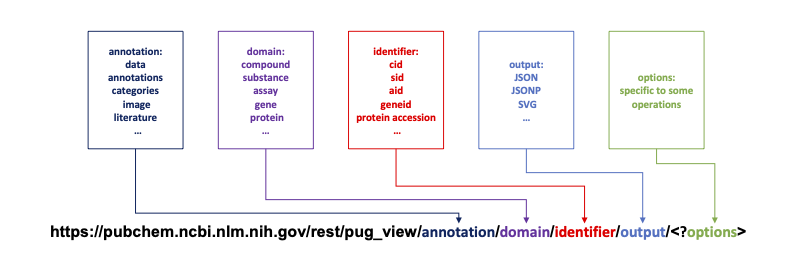
\includegraphics[width=1\linewidth,height=0.2\textheight]{figures/Figure_2} \caption{Using the PubChemR package to access PubChem's PUG-View database, with queries in URL syntax serving as function arguments}\label{fig:figure2}
\end{figure}

The \texttt{get\_pug\_view} function finds its application in various scenarios, making it a crucial resource in chemical data analysis:

\textbf{1. Full Data Record:} For researchers requiring comprehensive data of compounds, substances, or bioassays, \texttt{get\_pug\_view} provides detailed reports including experimental properties, safety information, and more.

We will initialize the retrieval of comprehensive data for the compound with ID 2244 (Aspirin) from PubChem using the following code chunk:

\begin{verbatim}
full_record_2244 <- get_pug_view(annotation = "data", 
                                 identifier = "2244", 
                                 domain = "compound", 
                                 output = "JSON") 
full_record_2244
\end{verbatim}

\begin{verbatim}
#> 
#>  PUG View Data from PubChem Database 
#> 
#>  Request Details:  
#>   - Domain: Compound
#>   - Annotation: data
#>   - Identifier: 2244
#> 
#>  Pug View Details: 
#>   - RecordType (1): [<unnamed character>] 
#>   - RecordNumber (1): [<unnamed numeric>] 
#>   - RecordTitle (1): [<unnamed character>] 
#>   - Section (20): [<unnamed list>] Structures, Chemical Safety, ... and 18 more.
#>   - Reference (243): [<unnamed list>] 
#> 
#>  NOTE: Run getter function 'retrieve()' with element name above to extract data from corresponding list. 
#>        See ?retrieve for details.
\end{verbatim}

The resulting object contains extensive information about the compound, including various sections and references.

We can extract the record type, record number, and record title to confirm that the record pertains to a chemical compound, to identify the specific compound ID for Aspirin, and to verify that Aspirin is the common name for the compound with ID 2244. Moreoveer, \texttt{retrieve} function can be used to show detailed information about the references, including reference number, source name, source ID, name, description, URL, and license URL. Each reference provides insights into various aspects related to the compound Aspirin, sourced from databases like the Australian Industrial Chemicals Introduction Scheme (AICIS), CAMEO Chemicals, CAS Common Chemistry, and others. These references include descriptions of the chemical properties, regulatory information, safety data, and links to the original sources for further details.

To access the specific sections within the retrieved data, we use the following code:

\begin{verbatim}
sections <- retrieve(object = full_record_2244, .slot = "Section")
sections
\end{verbatim}

\begin{verbatim}
#> 
#>  PUG View Data Sections 
#> 
#>  Request Details: 
#>   - Record Type: CID
#>   - Record Number: 2244
#>   - Record Title: Aspirin
#> 
#>  Section Details: 
#>   - Number of available sections: 20
#>   - Section headings: Structures, Chemical Safety, ... and 18 more.
#> 
#>  NOTE: Run getter function 'section()' to extract section data. To list available sections, run 'sectionList()'. 
#>        See ?section and ?sectionList for details.
\end{verbatim}

This code retrieves the sections available within the full record of Aspirin. The output indicates that there are 20 sections available, with headings such as Structures, Chemical Safety, and others.

Now, we can employ the \texttt{sectionList} function to display all sections available in the ``sections'' object:

\begin{verbatim}
sectionList(object = sections)
\end{verbatim}

\begin{verbatim}
#> # A tibble: 20 x 2
#>    SectionID Headings                         
#>    <chr>     <chr>                            
#>  1 S1        Structures                       
#>  2 S2        Chemical Safety                  
#>  3 S3        Names and Identifiers            
#>  4 S4        Chemical and Physical Properties 
#>  5 S5        Spectral Information             
#>  6 S6        Related Records                  
#>  7 S7        Chemical Vendors                 
#>  8 S8        Drug and Medication Information  
#>  9 S9        Pharmacology and Biochemistry    
#> 10 S10       Use and Manufacturing            
#> 11 S11       Identification                   
#> 12 S12       Safety and Hazards               
#> 13 S13       Toxicity                         
#> 14 S14       Associated Disorders and Diseases
#> 15 S15       Literature                       
#> 16 S16       Patents                          
#> 17 S17       Interactions and Pathways        
#> 18 S18       Biological Test Results          
#> 19 S19       Taxonomy                         
#> 20 S20       Classification
\end{verbatim}

The ``SectionID'' column contains unique identifiers for each section, labeled S1 through S20. The ``Headings'' column provides descriptive titles for these sections, indicating the type of information contained within each.

The sections listed are:

\textbf{1. Structures:} Details on the structural information of Aspirin.

\textbf{2. Chemical Safety:} Information related to the safety measures and regulations for handling Aspirin.

\textbf{3. Names and Identifiers:} Various names and identifiers associated with Aspirin.

\textbf{4. Chemical and Physical Properties:} Data on the chemical and physical properties of Aspirin.

\textbf{5. Spectral Information:} Spectral data related to Aspirin.

\textbf{6. Related Records:} Records related to Aspirin.

\textbf{7. Chemical Vendors:} Information about vendors that supply Aspirin.

\textbf{8. Drug and Medication Information:} Details on the use of Aspirin as a drug or medication.

\textbf{9. Pharmacology and Biochemistry:} Information on the pharmacological and biochemical properties of Aspirin.

\textbf{10. Use and Manufacturing:} Data on the use and manufacturing processes of Aspirin.

\textbf{11. Identification:} Identification information for Aspirin.

\textbf{12. Safety and Hazards:} Safety hazards associated with Aspirin.

\textbf{13. Toxicity:} Toxicological information about Aspirin.

\textbf{14. Associated Disorders and Diseases:} Disorders and diseases associated with Aspirin.

\textbf{15. Literature:} References to literature involving Aspirin.

\textbf{16. Patents:} Patent information related to Aspirin.

\textbf{17. Interactions and Pathways:} Biological interactions and pathways involving Aspirin.

\textbf{18. Biological Test Results:} Results from biological tests conducted on Aspirin.

\textbf{19. Taxonomy:} Taxonomic information related to Aspirin.

\textbf{20. Classification:} Classification information for Aspirin.

These sections provide a comprehensive overview of various aspects of Aspirin. Now, we will focus on detailed data from the first section, ``Structures,'' with the section ID ``S1''.

First, we assign the section to an object using the \texttt{section} function and then examine its contents:

\begin{verbatim}
s1 <- section(object = sections, .id = "S1")
\end{verbatim}

The output provides an overview of the ``Structures'' section:

\begin{verbatim}
s1
\end{verbatim}

\begin{verbatim}
#> 
#>  PUG View Data Sections (Structures) 
#> 
#>  Request Details: 
#>   - Record Type: CID
#>   - Record Number: 2244
#>   - Record Title: Aspirin
#> 
#>  Section Details: 
#>   - TOCHeading (1): [<unnamed character>] 
#>   - Description (1): [<unnamed character>] 
#>   - Section (3): [<unnamed list>] 2D Structure, 3D Conformer, ... and 1 more.
#> 
#>  NOTE: Run getter function 'retrieve()' with element name above to extract data from corresponding list. 
#>        See ?retrieve for details. 
#> 
#>  NOTE: Run getter function 'section()' to extract section data. To list available sections, run 'sectionList()'. 
#>        See ?section and ?sectionList for details.
\end{verbatim}

Next, we list the sub-sections within the ``Structures'' section. The output shows the available sub-sections:

\begin{verbatim}
sectionList(object = s1)
\end{verbatim}

\begin{verbatim}
#> # A tibble: 3 x 2
#>   SectionID Headings          
#>   <chr>     <chr>             
#> 1 S1        2D Structure      
#> 2 S2        3D Conformer      
#> 3 S3        Crystal Structures
\end{verbatim}

This breakdown allows us to see that the ``Structures'' section contains detailed depictions of Aspirin, including 2D structures, 3D conformers, and crystal structures. Each sub-section can be further explored to gain more specific information about the molecular structure of Aspirin.

\textbf{2. Accessing Specific Headings:} Users can retrieve data under specific headings for targeted information, such as boiling points or viscosity measurements.

First, we initiate the retrieval of data for a specific heading using the \texttt{get\_pug\_view} function, focusing on the ``Boiling Point'' heading within the ``heading'' domain.

\begin{verbatim}
specific_headings <- get_pug_view(annotation = "annotations", 
                                  identifier = "Boiling Point", 
                                  domain = "heading", 
                                  output = "JSON", 
                                  headingType = "Compound")

specific_headings
\end{verbatim}

\begin{verbatim}
#> 
#>  PUG View Data from PubChem Database 
#> 
#>  Request Details:  
#>   - Domain: DomainSpecific (heading)
#>   - Annotation: annotations
#>   - Identifier: Boiling%20Point
#> 
#>  Pug View Details: 
#>   - Annotation (1000): [<unnamed list>] 
#>   - Page (1): [<unnamed numeric>] 
#>   - TotalPages (1): [<unnamed numeric>] 
#> 
#>  NOTE: Run getter function 'retrieve()' with element name above to extract data from corresponding list. 
#>        See ?retrieve for details.
\end{verbatim}

The function call returns data from the PubChem database, specifying details about the request, including the domain, annotation type, identifier, and the number of annotations retrieved. It highlights that 1000 annotations were fetched, spread across multiple pages.

Next, we utilize the \texttt{retrieve} function to extract the ``Annotation'' slot from the \emph{specific\_headings} object. By displaying the annotations, we gain insight into the structure and content of the data. Each annotation includes the source name, source ID, compound name, description, URLs, and detailed data related to the boiling point, complete with references and specific values.

\begin{verbatim}
annotation <- retrieve(specific_headings, .slot = "Annotation", .to.data.frame = FALSE)
annotation[[1]]
\end{verbatim}

\begin{verbatim}
#> $SourceName
#> [1] "Hazardous Substances Data Bank (HSDB)"
#> 
#> $SourceID
#> [1] "30"
#> 
#> $Name
#> [1] "NITROGLYCERIN"
#> 
#> $Description
#> [1] "The Hazardous Substances Data Bank (HSDB) is a toxicology database that focuses on the toxicology of potentially hazardous chemicals. It provides information on human exposure, industrial hygiene, emergency handling procedures, environmental fate, regulatory requirements, nanomaterials, and related areas. The information in HSDB has been assessed by a Scientific Review Panel."
#> 
#> $URL
#> [1] "https://pubchem.ncbi.nlm.nih.gov/source/hsdb/30"
#> 
#> $LicenseURL
#> [1] "https://www.nlm.nih.gov/web_policies.html"
#> 
#> $Data
#> $Data[[1]]
#> $Data[[1]]$TOCHeading
#>            type     #TOCHeading 
#>      "Compound" "Boiling Point" 
#> 
#> $Data[[1]]$Description
#> [1] "PEER REVIEWED"
#> 
#> $Data[[1]]$Reference
#> [1] "O'Neil, M.J. (ed.). The Merck Index - An Encyclopedia of  Chemicals, Drugs, and Biologicals. 13th Edition, Whitehouse  Station, NJ:  Merck and Co., Inc., 2001., p. 1185"
#> 
#> $Data[[1]]$Value
#> $Data[[1]]$Value$StringWithMarkup
#> $Data[[1]]$Value$StringWithMarkup[[1]]
#>               String 
#> "Explodes at 218 °C" 
#> 
#> 
#> 
#> 
#> $Data[[2]]
#> $Data[[2]]$TOCHeading
#>            type     #TOCHeading 
#>      "Compound" "Boiling Point" 
#> 
#> $Data[[2]]$Description
#> [1] "PEER REVIEWED"
#> 
#> $Data[[2]]$Reference
#> [1] "Weast, R.C. (ed.) Handbook of Chemistry and Physics. 69th ed. Boca Raton, FL: CRC Press Inc., 1988-1989., p. C-291"
#> 
#> $Data[[2]]$Value
#> $Data[[2]]$Value$StringWithMarkup
#> $Data[[2]]$Value$StringWithMarkup[[1]]
#>                            String 
#> "BOILING POINT: 125 °C @ 2 MM HG" 
#> 
#> 
#> 
#> 
#> 
#> $ANID
#> [1] 2
#> 
#> $LinkedRecords
#> $LinkedRecords$CID
#> [1] 4510
\end{verbatim}

This step reveals detailed information about various compounds, including their boiling points. For instance, it might display data such as ``NITROGLYCERIN'' from the ``Hazardous Substances Data Bank (HSDB)'' with specific boiling point details like ``Explodes at 218 °C.''

\textbf{3. Literature and Publication Data:} The function can be used to retrieve literature associated with a compound, aiding in academic research and publication review.

In the given example, we are querying the PubChem database for literature information related to the compound with identifier ``1234'' in the compound domain. The identifier ``1234'' corresponds to the compound Gallopamil. Gallopamil is a pharmaceutical compound used primarily as a calcium channel blocker, which is useful in treating cardiovascular conditions such as angina pectoris and hypertension.

By running the \texttt{get\_pug\_view} function with the identifier ``1234'', we retrieve various details about Gallopamil, including references to related literature.

\begin{verbatim}
literature <- get_pug_view(annotation = "literature", 
                           identifier = "1234", 
                           domain = "compound", 
                           output = "JSON")
literature
\end{verbatim}

\begin{verbatim}
#> 
#>  PUG View Data from PubChem Database 
#> 
#>  Request Details:  
#>   - Domain: Compound
#>   - Annotation: literature
#>   - Identifier: 1234
#> 
#>  Pug View Details: 
#>   - RecordType (1): [<unnamed character>] 
#>   - RecordNumber (1): [<unnamed numeric>] 
#>   - AllURL (1): [<unnamed character>] 
#> 
#>  NOTE: Run getter function 'retrieve()' with element name above to extract data from corresponding list. 
#>        See ?retrieve for details.
\end{verbatim}

The following code provides a URL, which directs to the PubMed search page for the specified compound. This link is valuable for researchers seeking detailed literature information related to the compound identified by CID 1234.

\begin{verbatim}
retrieve(literature, .slot = "AllURL")
\end{verbatim}

\begin{verbatim}
#> # A tibble: 1 x 1
#>   value                                                                         
#>   <chr>                                                                         
#> 1 https://www.ncbi.nlm.nih.gov/sites/entrez?cmd=search&db=pubmed&term=%22Gallop~
\end{verbatim}

\textbf{4. 3D Protein Structures:} The \texttt{get\_pug\_view} function allows access to detailed 3D protein structure information associated with specific compounds. These 3D structures provide critical insights into the molecular interactions, mechanisms of action, and potential binding sites of compounds, which are essential for understanding their biological effects. Access to such detailed structural data aids in drug design, understanding enzyme mechanisms, and studying protein-ligand interactions. The visual representation of these structures, along with associated metadata like MMDB (Molecular Modeling Database) and PDB (Protein Data Bank) IDs, URLs for accessing detailed pages, and descriptions of the structures, further enhances the utility of this function in scientific research and development.

The following code retrieves a list of 3D protein structures associated with Aspirin (ID:2244):

\begin{verbatim}
list_3d_proteins <- get_pug_view(annotation = "structure", 
                                 identifier = "2244", 
                                 domain = "compound", 
                                 output = "JSON")
list_3d_proteins
\end{verbatim}

\begin{verbatim}
#> 
#>  PUG View Data from PubChem Database 
#> 
#>  Request Details:  
#>   - Domain: Compound
#>   - Annotation: structure
#>   - Identifier: 2244
#> 
#>  Pug View Details: 
#>   - RecordType (1): [<unnamed character>] 
#>   - RecordNumber (1): [<unnamed numeric>] 
#>   - URL (1): [<unnamed character>] 
#>   - NumberOfStructures (1): [<unnamed numeric>] 
#>   - Structures (8): [<unnamed list>] 
#> 
#>  NOTE: Run getter function 'retrieve()' with element name above to extract data from corresponding list. 
#>        See ?retrieve for details.
\end{verbatim}

This code fetches detailed information about the 3D protein structures related to Aspirin. The output includes several components.

First, the URL for the data is retrieved:

\begin{verbatim}
retrieve(list_3d_proteins, .slot = "URL")
\end{verbatim}

\begin{verbatim}
#> # A tibble: 1 x 1
#>   value                                                                         
#>   <chr>                                                                         
#> 1 https://www.ncbi.nlm.nih.gov/sites/entrez?LinkName=pccompound_structure&db=pc~
\end{verbatim}

This output provides the URL to the PubChem page that contains detailed information about the 3D structures of Aspirin. This URL can be visited to explore further details visually and interactively.

Next, the number of 3D structures available is retrieved:

\begin{verbatim}
retrieve(list_3d_proteins, .slot = "NumberOfStructures")
\end{verbatim}

\begin{verbatim}
#> # A tibble: 1 x 1
#>   value
#>   <dbl>
#> 1     8
\end{verbatim}

The output indicates that there are 8 different 3D structures available for Aspirin.

Finally, details of each structure are retrieved:

\begin{verbatim}
list_3d_proteins_structures <- retrieve(list_3d_proteins, .slot = "Structures", .to.data.frame = FALSE)
\end{verbatim}

This code outputs a list of details for each 3D structure, including the MMDB ID, PDB ID, URLs for accessing and visualizing the structures, descriptions, and taxonomic information. For example, one of the structures is described as ``Cryo-EM structure of aspirin-bound ABCC4,'' with the MMDB ID 230639 and PDB ID ``8J3W.'' The structure is associated with Homo sapiens (human) as indicated by the taxonomy information.

\begin{verbatim}
list_3d_proteins_structures[[1]]
\end{verbatim}

\begin{verbatim}
#> $MMDB_ID
#> [1] 230639
#> 
#> $PDB_ID
#> [1] "8J3W"
#> 
#> $URL
#> [1] "https://www.ncbi.nlm.nih.gov/Structure/mmdb/mmdbsrv.cgi?uid=230639"
#> 
#> $ImageURL
#> [1] "https://www.ncbi.nlm.nih.gov/Structure/mmdb/mmdbimage.fcgi?small=t&id=230639"
#> 
#> $Description
#> [1] "Cryo-EM structure of aspirin-bound ABCC4"
#> 
#> $Taxonomy
#> $Taxonomy$ID
#> [1] 9606
#> 
#> $Taxonomy$Name
#> [1] "Homo sapiens"
\end{verbatim}

\textbf{5. NCBI LinkOut Records:} The \texttt{get\_pug\_view} function is capable of listing all LinkOut records for substances, compounds, or assays, which is beneficial for tracking external resources and databases linked to specific chemical entities. This functionality is especially useful for researchers who need to access a wide array of related data from different external sources.

Here is an example of how the LinkOut records can be retrieved for identifier ``1234'':

\begin{verbatim}
ncbi_linkouts <- get_pug_view(annotation = "linkout", 
                              identifier = "1234", 
                              domain = "compound", 
                              output = "JSON")
\end{verbatim}

Next, the retrieved data can then be accessed as follows:

\begin{verbatim}
retrieve(ncbi_linkouts, .slot = "ObjUrl", .to.data.frame = FALSE)
\end{verbatim}

\begin{verbatim}
#> $Url
#> [1] "http://partnersolution.ingenuity.com/?cid=97ae3f91eab87a&p1=EntrezPubChem&p2=GV&s=&ipaUri=%2Fpa%2Fapi%2Fv2%2Fgeneview%3Fapplicationname%3DEntrezPubChem%26geneId%3DING:qkb%26geneidtype%3Dingenuity"
#> 
#> $SubjectType
#> [1] "molecular interactions"
#> 
#> $Category
#> [1] "Chemical Information"
#> 
#> $Attribute
#> [1] "subscription/membership/fee required"
#> 
#> $Provider
#>                          Name                      NameAbbr 
#> "Ingenuity Pathways Analysis"                   "Ingenuity" 
#>                            Id                           Url 
#>                        "5628"    "http://www.ingenuity.com"
\end{verbatim}

The extracted data includes information such as the URL of the external resource, the subject type, the category of information, attributes indicating if a subscription or fee is required, and the provider's details. For instance, the URL ``\url{http://partnersolution.ingenuity.com/?cid=97ae3f91eab87a\&p1=EntrezPubChem\&p2=GV\&s=\&ipaUri=\%2Fpa\%2Fapi\%2Fv2\%2Fgeneview\%3Fapplicationname\%3DEntrezPubChem\%26geneId\%3DING:qkb\%26geneidtype\%3Dingenuity}'' points to a resource provided by Ingenuity Pathways Analysis, categorized under ``Chemical Information'' and related to ``molecular interactions''. This URL requires a subscription or membership for access.

Such detailed LinkOut records facilitate the exploration of interconnected data across various platforms, enabling researchers to efficiently gather comprehensive information related to their chemical entities of interest.

\hypertarget{discussion}{%
\section{Discussion}\label{discussion}}

\hypertarget{related-packages}{%
\subsection{Related Packages}\label{related-packages}}

Several R packages provide access to chemical data and tools for cheminformatics, each with its unique focus and capabilities:

\begin{itemize}
\item
  \textbf{\BIOpkg{ChemmineR}:} A comprehensive cheminformatics toolkit for R, offering functionalities for compound data processing and analysis. It includes tools for compound classification, similarity searching, and structure-activity relationship modeling.
\item
  \textbf{\CRANpkg{webchem}:} Designed for retrieving chemical information from various web sources, this package facilitates automated queries and integrates data into R objects for further analysis, focusing on structured data retrieval and usage.
\item
  \textbf{\CRANpkg{rcdk}:} An R interface to the CDK, allowing users to manipulate and analyze chemical data. This package supports molecular structure parsing, descriptor calculation, and fingerprint generation, making it invaluable for computational chemistry, drug discovery, and bioinformatics research.
\item
  \textbf{\BIOpkg{ChemmineOB}:} An interface with OpenBabel for chemical format conversions and molecular property calculations, enhancing cheminformatics workflows by offering easy access to OpenBabel's powerful functions directly from R.
\item
  \textbf{\BIOpkg{BridgeDbR}:} Provides access to the BridgeDb framework, facilitating identifier mapping across different biological databases and supporting a wide range of identifier types, which is particularly useful in systems biology, genomics, and metabolomics studies.
\item
  \textbf{\BIOpkg{RMassBank}:} Tailored for the creation and handling of mass spectrometry databases, providing tools for building, querying, and managing MassBank records essential for compound identification and annotation in MS experiments.
\item
  \textbf{\BIOpkg{rgoslin}:} An R package for the systematic annotation of lipid species using the GOSlin format, supporting the conversion of lipid names to a structured format and ensuring consistency and accuracy in lipidomics studies.
\end{itemize}

\CRANpkg{PubChemR}, in comparison, is designed specifically to interface with the PubChem database, providing a focused approach for accessing chemical data within this database through R. While \BIOpkg{ChemmineR} and \CRANpkg{webchem} offer broad functionalities and access to multiple sources, \CRANpkg{PubChemR} specializes in efficient and targeted data interactions with PubChem, making it particularly suitable for users who predominantly rely on PubChem for their chemical data needs.

In the Python ecosystem, libraries such as \pkg{PubChempy} (Swain 2017), \pkg{ChemSpiPy} (Swain 2018), and \pkg{CIRpy} (Swain 2016) offer functionalities similar to those described here. PubChemPy, like \CRANpkg{PubChemR}, provides a direct interface with the PubChem database for accessing chemical molecules and their properties, supporting various chemical searches, standardization, format conversions, depiction, and property retrieval. ChemSpiPy offers easy access to the ChemSpider web service, enabling chemical searches, downloads, and property retrieval. CIRpy interfaces with the Chemical Identifier Resolver (CIR) by the Computer-Aided Drug Design (CADD) Group at the National Cancer Institute (NCI), simplifying the conversion of chemical identifiers and calculation of properties, along with supporting diverse file format downloads.

\hypertarget{usage-policy-of-pug-rest-service}{%
\subsection{Usage Policy of PUG REST Service}\label{usage-policy-of-pug-rest-service}}

Please note that PUG REST is not intended for handling very large volumes of requests, such as those numbering in the millions. To prevent overloading the PubChem servers, it is requested that any script or application limit the request rate to no more than five requests per second. This measure helps ensure the stability and reliability of the service for all users. For more information on request volume limitations and automated rate limiting (throttling), please refer to PubChem's dynamic request throttling documentation (\url{https://pubchem.ncbi.nlm.nih.gov/docs/dynamic-request-throttling}).

In some cases, a 503 HTTP status code may be returned when the server is temporarily unable to service the request due to maintenance downtime or capacity issues. If this occurs, it is advisable to try the request again later. This status code indicates that the server is currently overloaded or undergoing maintenance, and retrying the request after some time should allow it to be processed successfully.

\hypertarget{furter-research}{%
\subsection{Furter Research}\label{furter-research}}

The primary contribution of \CRANpkg{PubChemR} is its facilitation of direct access to PubChem's chemical data through the R programming environment. This functionality addresses a specific need for researchers who rely on R for data analysis and representation, allowing for more straightforward integration of chemical data into their workflows However, the effectiveness of \CRANpkg{PubChemR} is closely tied to the quality and comprehensiveness of the PubChem database. Inaccuracies or gaps in the PubChem data directly impact the outputs of \CRANpkg{PubChemR}, which is an important consideration for users relying on this tool for research or data analysis. As PubChem's database is dynamic and continually updated, keeping \CRANpkg{PubChemR} synchronized with these updates is critical for maintaining its accuracy and relevance.

While \CRANpkg{PubChemR} currently focuses on accessing PubChem data and does not include data analysis functions, future enhancements could potentially explore these areas. For instance, more sophisticated data analysis capabilities within the package itself could be developed, enabling users to perform preliminary analysis within the same framework. Another possible direction could be the integration with other chemical databases, expanding the range of accessible data. Additionally, improving the user interface for greater ease of use and better data visualization capabilities could make the tool more accessible to a wider range of users with varying levels of expertise in R programming. These are potential directions for future research and development, although there are no immediate plans to implement these features.

\hypertarget{summary}{%
\section{Summary}\label{summary}}

\CRANpkg{PubChemR} represents a significant advancement in accessing chemical data through the R programming environment. It offers a straightforward, effective, and easy-to-use way to access information from the PubChem database, improving how users can get chemical data. \CRANpkg{PubChemR} combines practical features with user-friendly design, making it a useful tool for researchers in various scientific areas. As it continues to receive updates and enhancements, \CRANpkg{PubChemR} will keep up with changes in chemical data and computational technology.

\hypertarget{references}{%
\section*{References}\label{references}}
\addcontentsline{toc}{section}{References}

\hypertarget{refs}{}
\begin{CSLReferences}{1}{0}
\leavevmode\vadjust pre{\hypertarget{ref-cao2008chemminer}{}}%
Cao, Yiqun, Anna Charisi, Li-Chang Cheng, Tao Jiang, and Thomas Girke. 2008. {``ChemmineR: A Compound Mining Framework for r.''} \emph{Bioinformatics} 24 (15): 1733--34.

\leavevmode\vadjust pre{\hypertarget{ref-chen2009pubchem}{}}%
Chen, Bin, David Wild, and Rajarshi Guha. 2009. {``PubChem as a Source of Polypharmacology.''} \emph{Journal of Chemical Information and Modeling} 49 (9): 2044--55.

\leavevmode\vadjust pre{\hypertarget{ref-guha2007chemical}{}}%
Guha, Rajarshi. 2007. {``Chemical Informatics Functionality in r.''} \emph{Journal of Statistical Software} 18: 1--16.

\leavevmode\vadjust pre{\hypertarget{ref-horan2024}{}}%
Horan, Kevin, and Thomas Girke. 2024. \emph{ChemmineOB: R Interface to a Subset of OpenBabel Functionalities}. \url{https://www.bioconductor.org/packages/release/bioc/html/ChemmineOB.html}.

\leavevmode\vadjust pre{\hypertarget{ref-kim2015pug}{}}%
Kim, Sunghwan, Paul A Thiessen, Evan E Bolton, and Stephen H Bryant. 2015. {``PUG-SOAP and PUG-REST: Web Services for Programmatic Access to Chemical Information in PubChem.''} \emph{Nucleic Acids Research} 43 (W1): W605--11.

\leavevmode\vadjust pre{\hypertarget{ref-kim2016pubchem}{}}%
Kim, Sunghwan, Paul A Thiessen, Evan E Bolton, Jie Chen, Gang Fu, Asta Gindulyte, Lianyi Han, et al. 2016. {``PubChem Substance and Compound Databases.''} \emph{Nucleic Acids Research} 44 (D1): D1202--13.

\leavevmode\vadjust pre{\hypertarget{ref-kim2018update}{}}%
Kim, Sunghwan, Paul A Thiessen, Tiejun Cheng, Bo Yu, and Evan E Bolton. 2018. {``An Update on PUG-REST: RESTful Interface for Programmatic Access to PubChem.''} \emph{Nucleic Acids Research} 46 (W1): W563--70.

\leavevmode\vadjust pre{\hypertarget{ref-kim2019pug}{}}%
Kim, Sunghwan, Paul A Thiessen, Tiejun Cheng, Jian Zhang, Asta Gindulyte, and Evan E Bolton. 2019. {``PUG-View: Programmatic Access to Chemical Annotations Integrated in PubChem.''} \emph{Journal of Cheminformatics} 11 (1): 1--11.

\leavevmode\vadjust pre{\hypertarget{ref-kopczynski2020goslin}{}}%
Kopczynski, Dominik, Nils Hoffmann, Bing Peng, and Robert Ahrends. 2020. {``Goslin: A Grammar of Succinct Lipid Nomenclature.''} \emph{Analytical Chemistry} 92 (16): 10957--60.

\leavevmode\vadjust pre{\hypertarget{ref-korkmaz2020deep}{}}%
Korkmaz, Selcuk. 2020. {``Deep Learning-Based Imbalanced Data Classification for Drug Discovery.''} \emph{Journal of Chemical Information and Modeling} 60 (9): 4180--90.

\leavevmode\vadjust pre{\hypertarget{ref-Korkmaz2024}{}}%
Korkmaz, Selcuk, Bilge Eren Yamasan, and Dincer Goksuluk. 2024. \emph{PubChemR: Interface to the 'PubChem' Database for Chemical Data Retrieval}. \url{https://CRAN.R-project.org/package=PubChemR}.

\leavevmode\vadjust pre{\hypertarget{ref-leemans2018}{}}%
Leemans, C, E Willighagen, A Bohler, and L Eijssen. 2024. \emph{BridgeDbR: Code for Using BridgeDb Identifier Mapping Framework from Within r}. \url{https://www.bioconductor.org/packages/release/bioc/html/BridgeDbR.html}.

\leavevmode\vadjust pre{\hypertarget{ref-li2010pubchem}{}}%
Li, Qingliang, Tiejun Cheng, Yanli Wang, and Stephen H Bryant. 2010. {``PubChem as a Public Resource for Drug Discovery.''} \emph{Drug Discovery Today} 15 (23-24): 1052--57.

\leavevmode\vadjust pre{\hypertarget{ref-stravs2013automatic}{}}%
Stravs, Michael A, Emma L Schymanski, Heinz P Singer, and Juliane Hollender. 2013. {``Automatic Recalibration and Processing of Tandem Mass Spectra Using Formula Annotation.''} \emph{Journal of Mass Spectrometry} 48 (1): 89--99.

\leavevmode\vadjust pre{\hypertarget{ref-swain2016cirpy}{}}%
Swain, Matt. 2016. \emph{CIRpy: Python Wrapper for the NCI Chemical Identifier Resolver}. \url{https://github.com/mcs07/CIRpy}.

\leavevmode\vadjust pre{\hypertarget{ref-swain2014pubchempy}{}}%
---------. 2017. \emph{PubChemPy: Python Wrapper for the PubChem PUG REST API}. \url{https://github.com/mcs07/PubChemPy}.

\leavevmode\vadjust pre{\hypertarget{ref-swain2012chemspipy}{}}%
---------. 2018. \emph{ChemSpiPy-a Python Wrapper for the ChemSpider API}. \url{https://github.com/mcs07/ChemSpiPy}.

\leavevmode\vadjust pre{\hypertarget{ref-szocs2020webchem}{}}%
Szöcs, Eduard, Tamás Stirling, Eric R Scott, Andreas Scharmüller, and Ralf B Schäfer. 2020. {``Webchem: An r Package to Retrieve Chemical Information from the Web.''} \emph{Journal of Statistical Software} 93: 1--17.

\leavevmode\vadjust pre{\hypertarget{ref-wang2009pubchem}{}}%
Wang, Yanli, Jewen Xiao, Tugba O Suzek, Jian Zhang, Jiyao Wang, and Stephen H Bryant. 2009. {``PubChem: A Public Information System for Analyzing Bioactivities of Small Molecules.''} \emph{Nucleic Acids Research} 37 (suppl\_2): W623--33.

\leavevmode\vadjust pre{\hypertarget{ref-wang2012pubchem}{}}%
Wang, Yanli, Jewen Xiao, Tugba O Suzek, Jian Zhang, Jiyao Wang, Zhigang Zhou, Lianyi Han, et al. 2012. {``PubChem's BioAssay Database.''} \emph{Nucleic Acids Research} 40 (D1): D400--412.

\leavevmode\vadjust pre{\hypertarget{ref-yamasan2024binding}{}}%
Yamasan, Bilge Eren, and Selçuk Korkmaz. 2024. {``Binding Activity Classification of Anti-SARS-CoV-2 Molecules Using Deep Learning Across Multiple Assays.''} \emph{Balkan Medical Journal} 41 (3): 186.

\end{CSLReferences}

\bibliography{RJreferences.bib}

\address{%
Selcuk Korkmaz\\
Trakya University\\%
Department Biostatistics\\ Edirne, Türkiye\\
%
%
\textit{ORCiD: \href{https://orcid.org/0000-0003-4632-6850}{0000-0003-4632-6850}}\\%
\href{mailto:selcukkorkmaz@trakya.edu.tr}{\nolinkurl{selcukkorkmaz@trakya.edu.tr}}%
}

\address{%
Bilge Eren Yamasan\\
Trakya University\\%
Department Biophysics\\ Edirne, Türkiye\\
%
%
\textit{ORCiD: \href{https://orcid.org/0000-0002-6525-2503}{0000-0002-6525-2503}}\\%
\href{mailto:berenyamasan@trakya.edu.tr}{\nolinkurl{berenyamasan@trakya.edu.tr}}%
}

\address{%
Dincer Goksuluk\\
Erciyes University\\%
Department Biostatistics\\ Kayseri, Türkiye\\
%
%
\textit{ORCiD: \href{https://orcid.org/0000-0002-2752-7668}{0000-0002-2752-7668}}\\%
\href{mailto:dincergoksuluk@erciyes.edu.tr}{\nolinkurl{dincergoksuluk@erciyes.edu.tr}}%
}
